\chapter{Realization}

\section{Introduction}

This chapter presents the realization of the AgriConnect system, translating the conceptual design and architecture defined in the previous chapter into a fully functional solution.

The implementation phase covers several key aspects of the system, including the setup of the development environment, the deployment of the database structure, and the integration of external services. In particular, the system relies on Supabase for data management and storage, and integrates WhatsApp as the primary communication channel to ensure accessibility for farmers.

A central component of the implementation is the use of automated workflows, developed using n8n, which handle message reception, processing, orchestration, and knowledge base ingestion. For example, the message reception workflow manages incoming WhatsApp messages, verifies user existence, processes different media types, and stores structured data for further processing. :contentReference[oaicite:0]{index=0}

In addition, the system incorporates a multi-agent architecture where each agent is responsible for a specific task, such as message normalization, orchestration, information retrieval, vision-based analysis, and escalation handling.

The chapter also presents the implementation of the web application, which provides dedicated interfaces for different types of users, including farmers, agronomists, administrators, and visitors. This interface complements the WhatsApp interaction by offering advanced functionalities such as case tracking, management, and system supervision.

Finally, the chapter introduces the knowledge base implementation, which enables the system to store, process, and retrieve agricultural information efficiently through vector-based search mechanisms. :contentReference[oaicite:1]{index=1}

Overall, this chapter demonstrates how the different components of AgriConnect are implemented and integrated to deliver a coherent and intelligent agricultural support platform.

\section{Development Environment and Tools}

\section{Database Implementation}

\section{WhatsApp Integration}

\section{Workflow Implementation}

\subsection{W00 — Message Reception Workflow}

\subsection{W01 — Orchestrator Workflow}

\subsection{Vision Sub-Workflow}

\subsection{KB Ingestion Workflow}

\section{Multi-Agent System Implementation}

\subsection{Normalizer Agent}

\subsection{Orchestrator Agent}

\subsection{RAG Agent}

\subsection{Vision Agent}

\subsection{Weather Agent}

\subsection{Escalation Agent}


\section{Web Application}

\subsection{Web Application Overview}

The AgriConnect web application is a central component of the platform, providing a structured interface that complements the WhatsApp-based interaction system. While WhatsApp ensures accessibility and ease of communication, the web application enables advanced functionalities such as case management, user interaction, and platform administration.

The platform is designed to support multiple types of users, each with specific roles:

\begin{itemize}
    \item \textbf{Visitors:} non-authenticated users who can access public pages of the platform. The visitor interface presents the objectives and features of AgriConnect, along with demonstration videos illustrating the farmer and agronomist interfaces. This interface serves as an entry point for new users.
    
    \item \textbf{Farmers:} users who can create agricultural cases manually through the web application. They are able to describe their issues, upload related media, track the evolution of their cases, and interact with agronomists through proposals and feedback.
    
    \item \textbf{Agronomists:} experts who can browse open cases that are not yet assigned. They can submit proposals to assist farmers, and once a proposal is accepted, they become responsible for the corresponding case and can provide detailed recommendations.
    
    \item \textbf{Administrators:} users responsible for managing the overall platform. They can supervise users, monitor cases, manage proposals, and review feedback to ensure proper system functioning.
\end{itemize}

The web application acts as a centralized interface for managing all platform activities. It allows users to visualize agricultural cases, access associated media, and follow interactions between farmers and agronomists.

Unlike the WhatsApp interface, which focuses on simplicity and quick communication, the web platform provides a more comprehensive and structured environment, enabling efficient case handling and system supervision.

The application is connected to backend services through APIs, ensuring real-time synchronization of data such as users, cases, proposals, and feedback. This guarantees consistency across all components of the AgriConnect system.

Overall, the web application enhances the platform by offering role-specific interfaces and advanced functionalities, making it an essential tool for effective agricultural support and collaboration.

\subsection{Global Application Architecture}

The AgriConnect web platform follows a multi-tier architecture based on a clear separation between the frontend, backend, and data storage layers. This design ensures scalability, maintainability, and flexibility in the system.

At the frontend level, the platform is composed of two distinct web applications developed using Next.js:

\begin{itemize}
    \item \textbf{Main Web Application:} accessible at \texttt{http://localhost:3000}, dedicated to visitors, farmers, and agronomists. It provides interfaces for case creation, case management, and interaction between users.
    
    \item \textbf{Admin Dashboard:} accessible at \texttt{http://localhost:3001}, a separate application designed specifically for administrators to manage users, monitor cases, and supervise platform activity.
\end{itemize}

Although these applications are deployed independently, they share the same backend services and communicate with the system through a common set of RESTful APIs.

The backend is implemented using Spring Boot and runs at \texttt{http://localhost:8081}. It exposes multiple endpoints such as \texttt{/api/users} and \texttt{/api/cases}, which handle business logic, data processing, and system operations. Both frontend applications interact with these endpoints to retrieve and update data in real time.

Authentication and authorization are handled through a hybrid approach combining Supabase authentication services and backend security mechanisms. This ensures secure access control and proper management of user roles across the platform.

For data storage, the system relies on Supabase, which provides both a relational database (PostgreSQL) and object storage for handling media files such as images associated with agricultural cases and user avatars.

The overall communication flow is based on REST API exchanges between the frontend applications and the backend. User actions performed in the interfaces (such as creating a case or submitting a proposal) trigger API requests, which are processed by the backend and reflected in the database.

This architecture allows both web applications to remain independent in terms of deployment while maintaining a unified and consistent interaction with the backend system.

\begin{figure}[H]
\centering
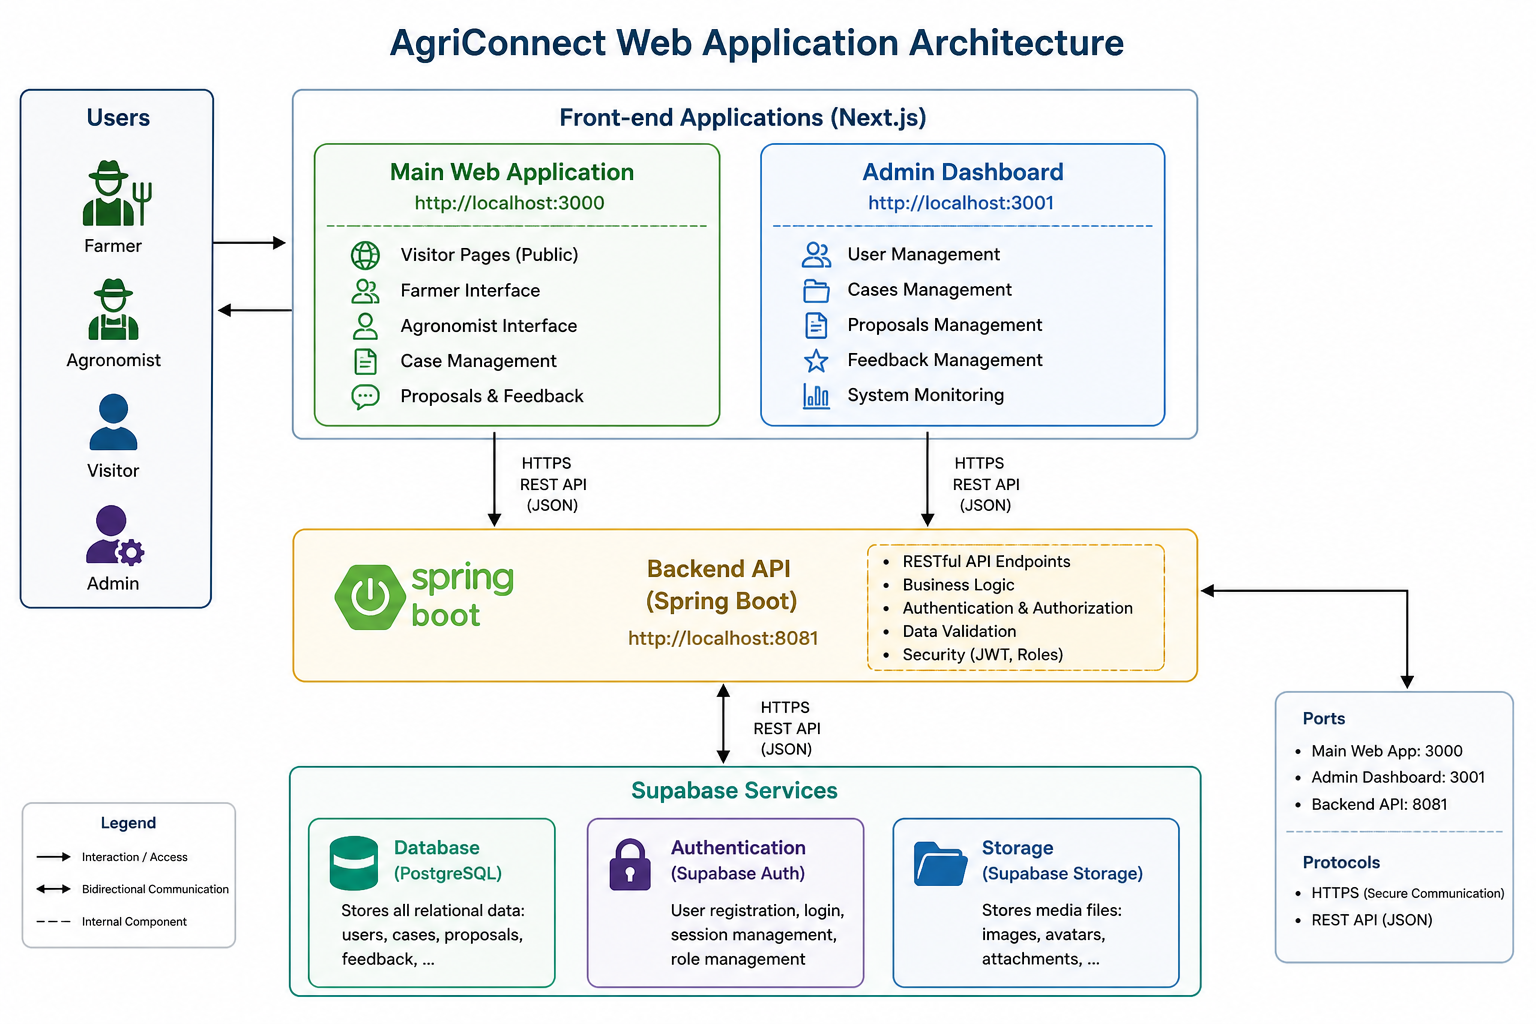
\includegraphics[width=0.9\textwidth]{images/diagrammes/webapp_architecture.png}
\caption{Global architecture of the AgriConnect web application}
\end{figure}

\subsection{Visitor Interface}

The visitor interface represents the public entry point of the AgriConnect web application. It is accessible without authentication and is designed to introduce the platform, explain its functionalities, and encourage users to register.

The main objective of this interface is to provide a clear understanding of the system and its value, particularly for farmers and agronomists who may not yet be familiar with digital agricultural solutions.

The visitor interface is structured into several main pages:

\begin{itemize}
    \item \textbf{Home Page:} This is the primary landing page of the application. It presents an overview of the AgriConnect platform, its objectives, and its key features. The page is designed to be visually clear and engaging, allowing users to quickly understand the purpose of the system.

    \begin{figure}[H]
    \centering
    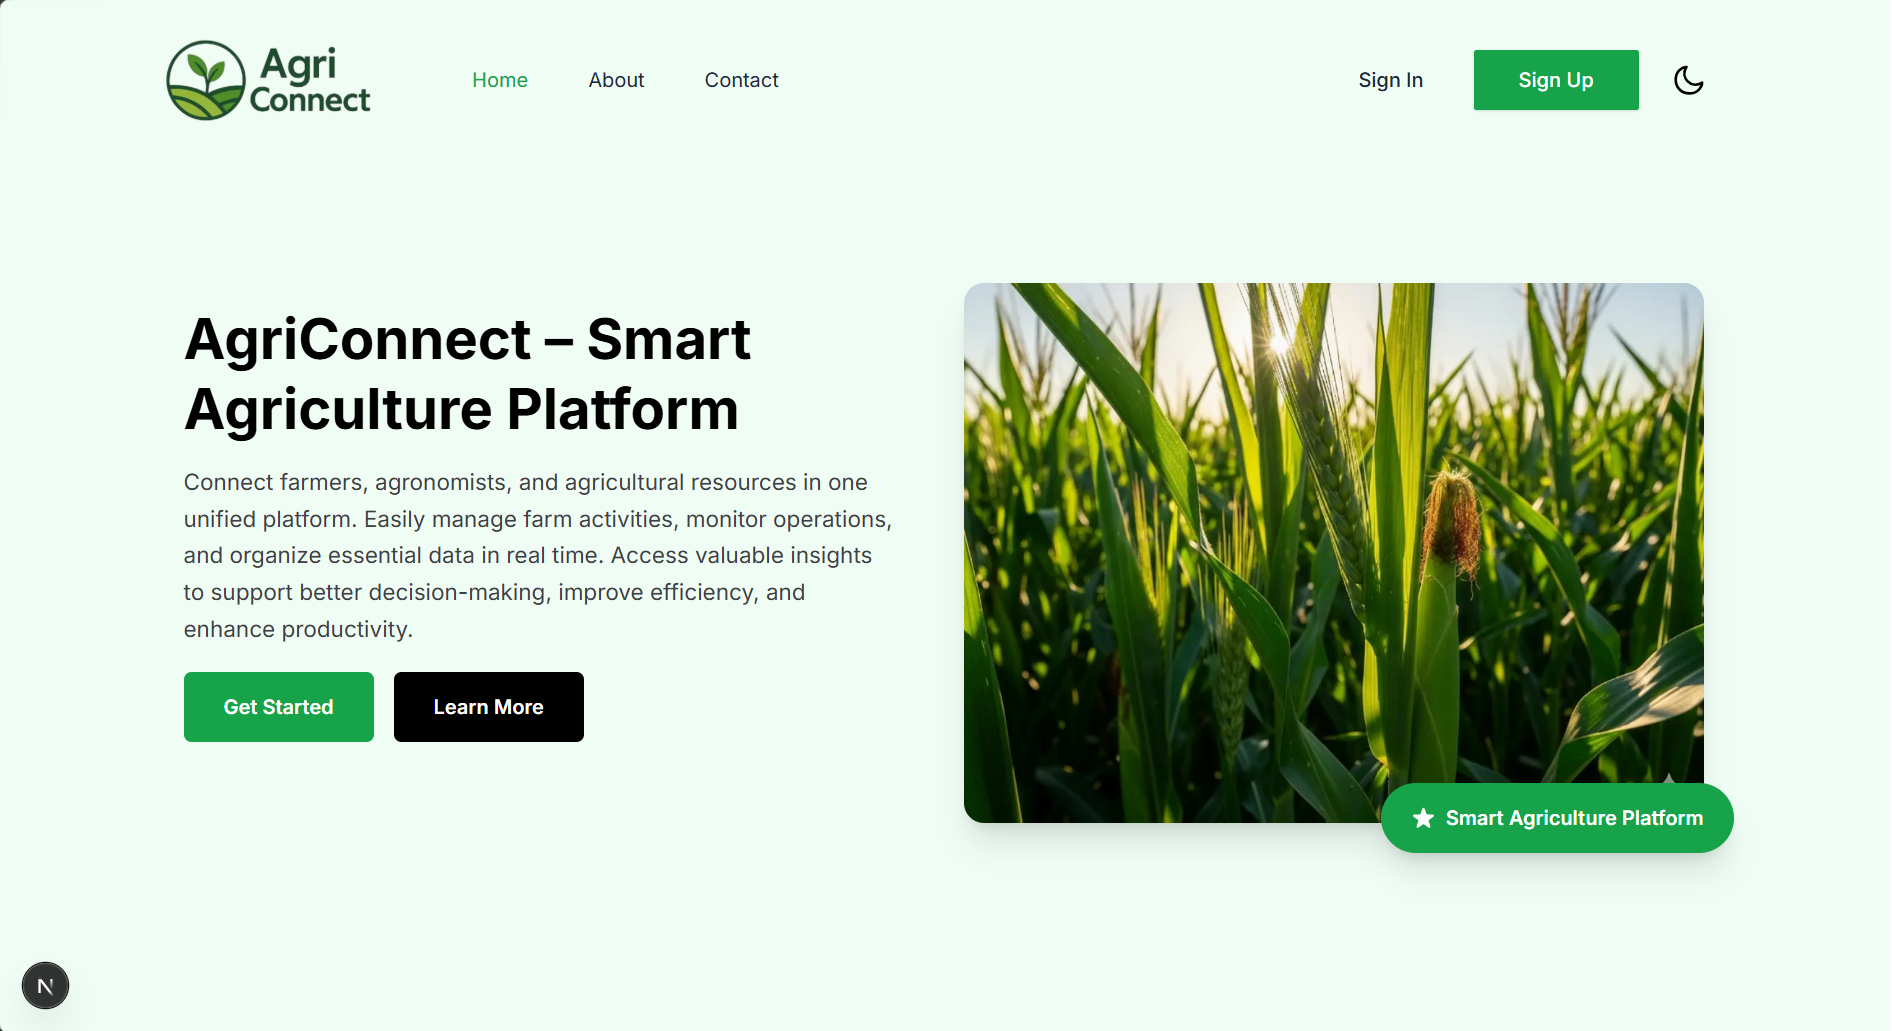
\includegraphics[width=0.9\textwidth]{images/interfaces/visitors/visitor_home.png}
    \caption{Home page of the AgriConnect visitor interface}
    \end{figure}

    \item \textbf{About Page:} This page provides detailed information about the platform, including its vision, functionalities, and the problems it aims to solve in the agricultural domain.

    \item \textbf{Contact Page:} This section allows users to access contact information or submit inquiries, enabling communication with the platform administrators.

    \item \textbf{Authentication Pages (Login / Register):} These pages allow users to create an account or log into the platform. The registration process is a key step for accessing the system’s functionalities, such as case creation and interaction with agronomists.
\end{itemize}

In addition to these pages, the visitor interface includes a demonstration component in the form of a video. This video illustrates how the platform is used, showcasing both the farmer and agronomist interfaces. It plays an important role in helping users understand the workflow of the system before registering.

\begin{figure}[H]
\centering
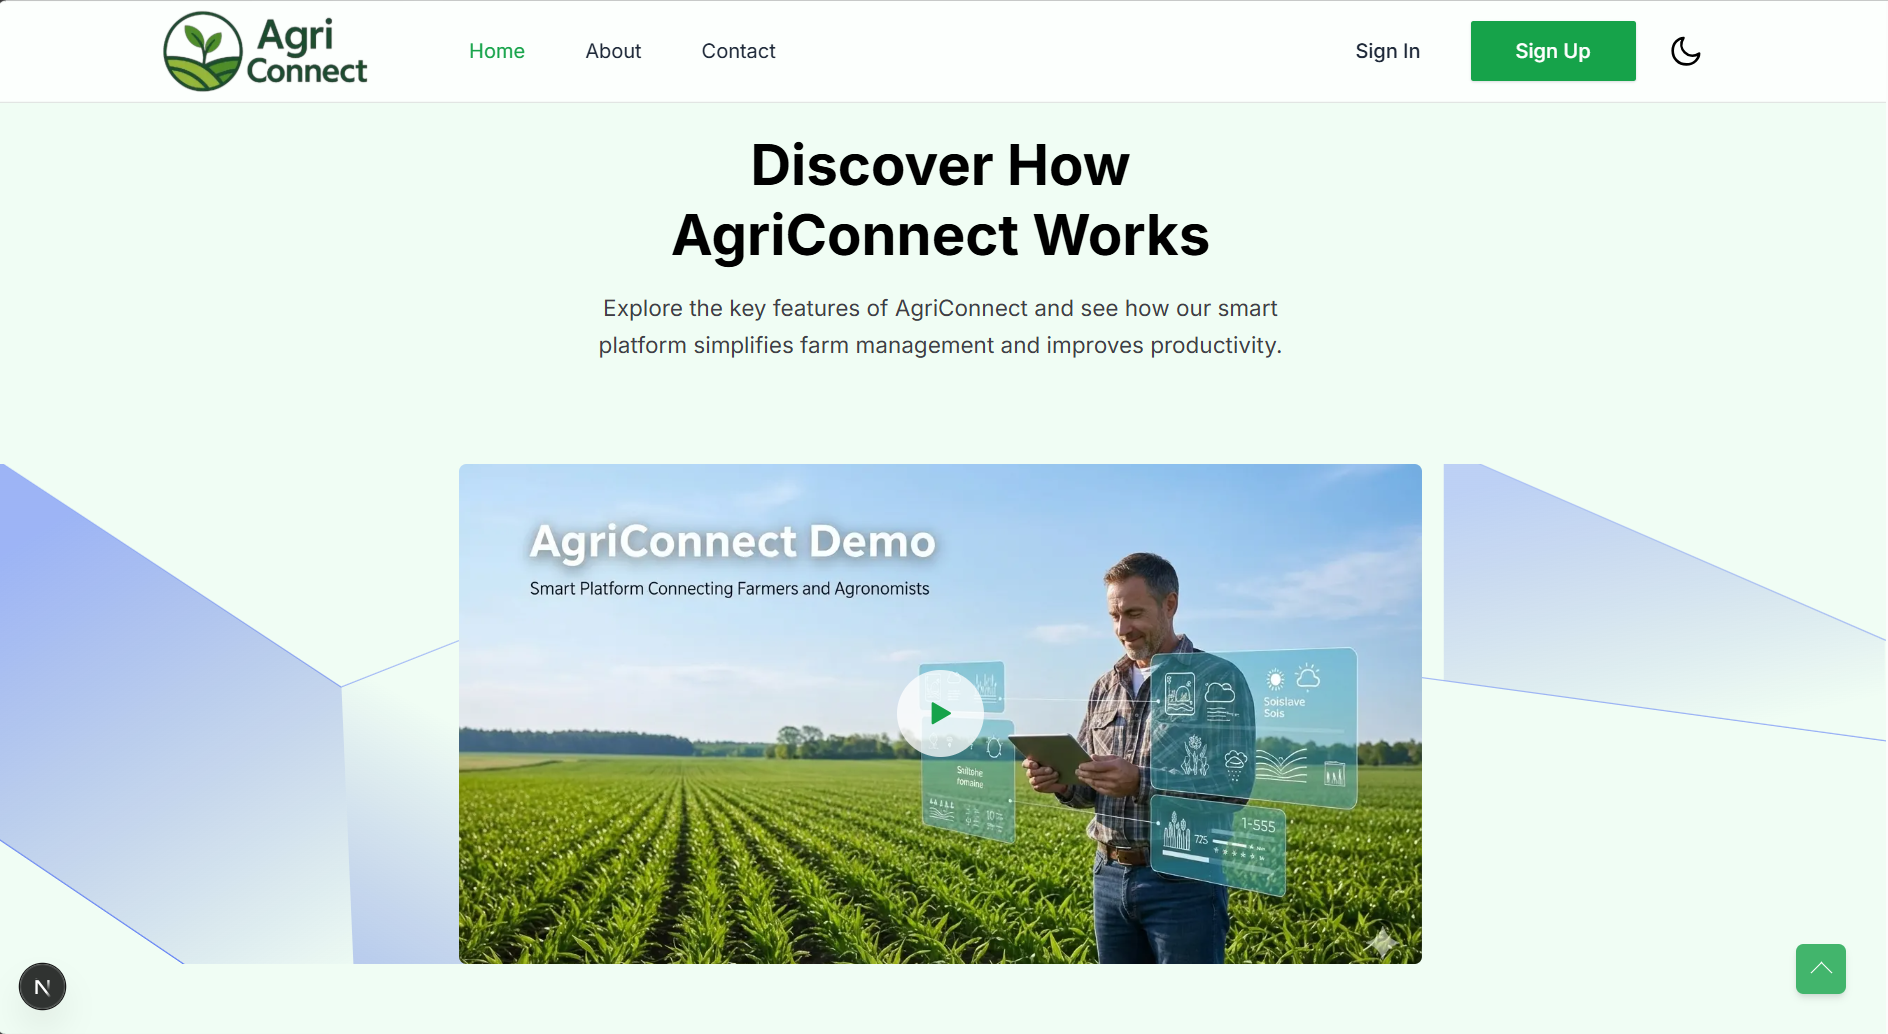
\includegraphics[width=0.9\textwidth]{images/interfaces/visitors/visitor_demo.png}
\caption{Demonstration video explaining the usage of the platform}
\end{figure}

From a design perspective, the interface is built using a modern frontend framework (Next.js) combined with a utility-first CSS approach (Tailwind CSS). The design focuses on clarity, simplicity, and responsiveness, ensuring accessibility across different devices, including mobile phones.

Overall, the visitor interface serves as an essential onboarding layer, guiding new users, explaining the platform’s capabilities, and facilitating their transition toward becoming active users of AgriConnect.

\subsection{Authentication and Role-Based Access}

Authentication and authorization are essential components of the AgriConnect web application, ensuring secure access to platform functionalities and proper separation of user responsibilities.

\subsubsection*{Authentication Mechanism}

The authentication process is based on email and password credentials using Supabase Authentication services. Users can create an account or log into the system through dedicated interfaces.

\begin{figure}[H]
\centering
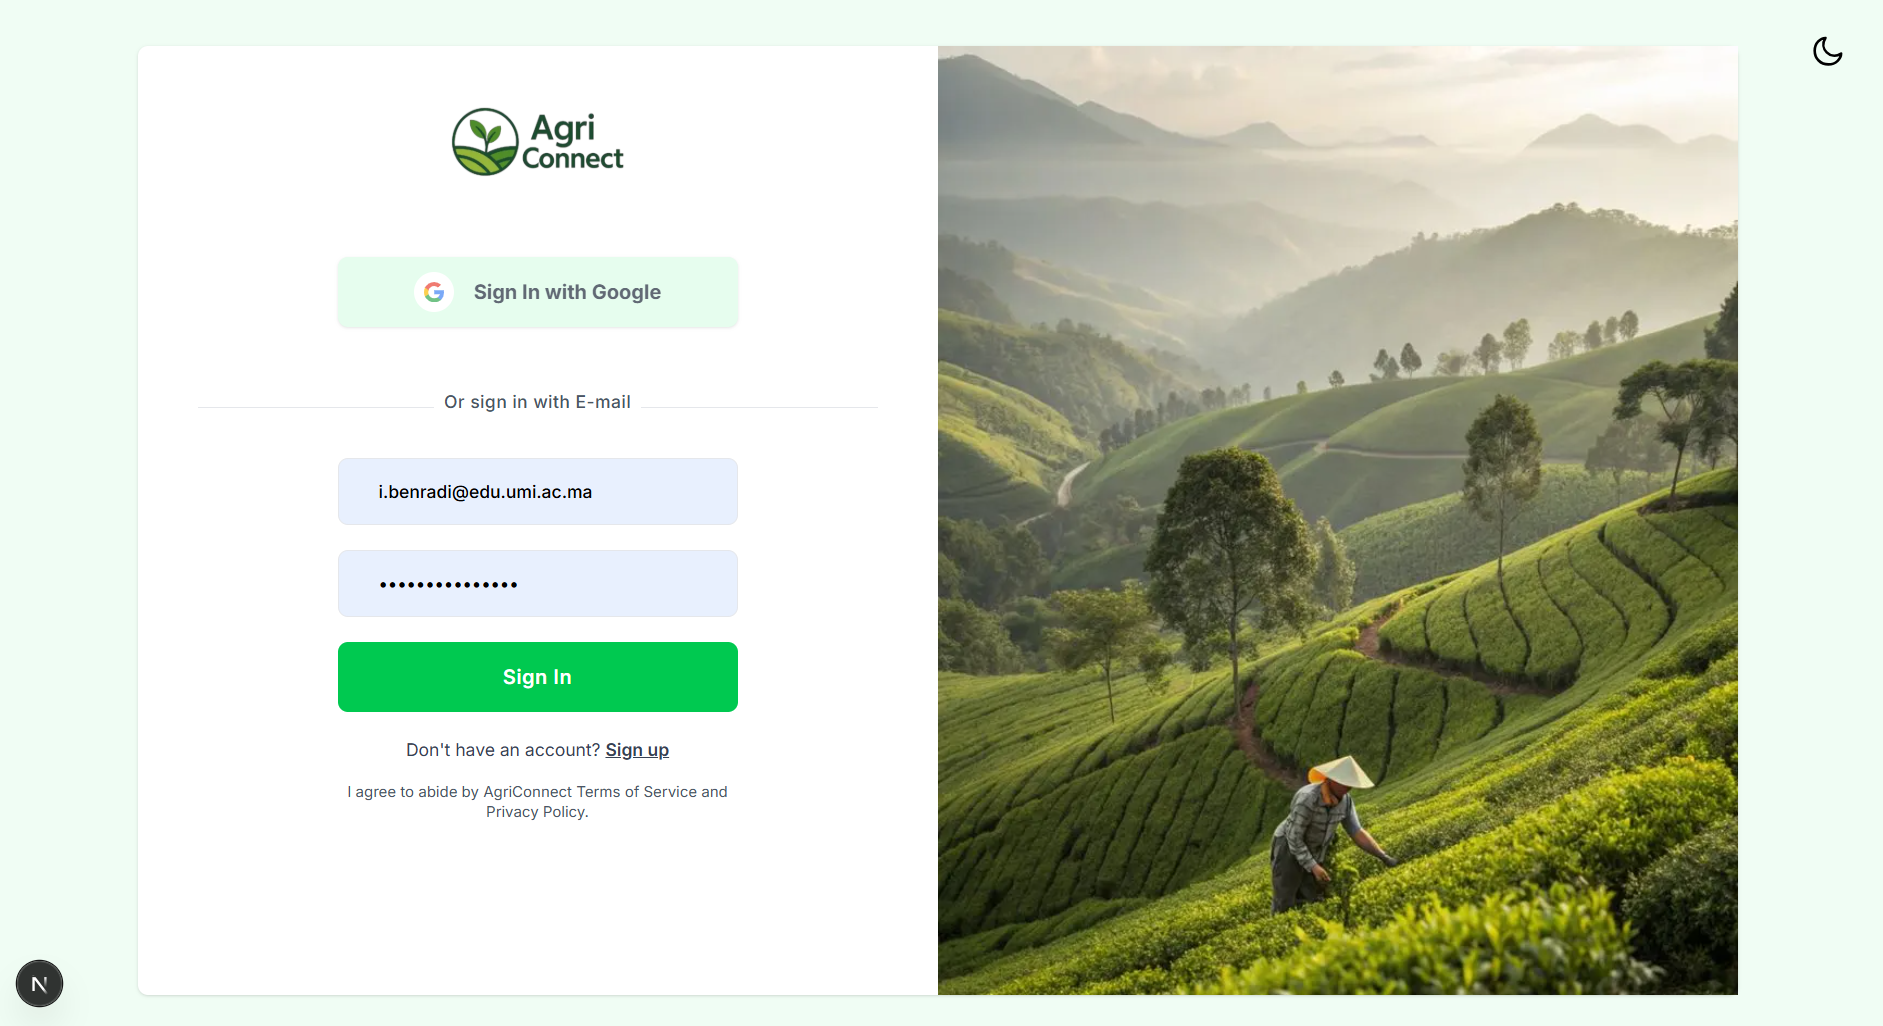
\includegraphics[width=0.8\textwidth]{images/interfaces/visitors/login_page.png}
\caption{Login page of the AgriConnect web application}
\end{figure}

\begin{figure}[H]
\centering
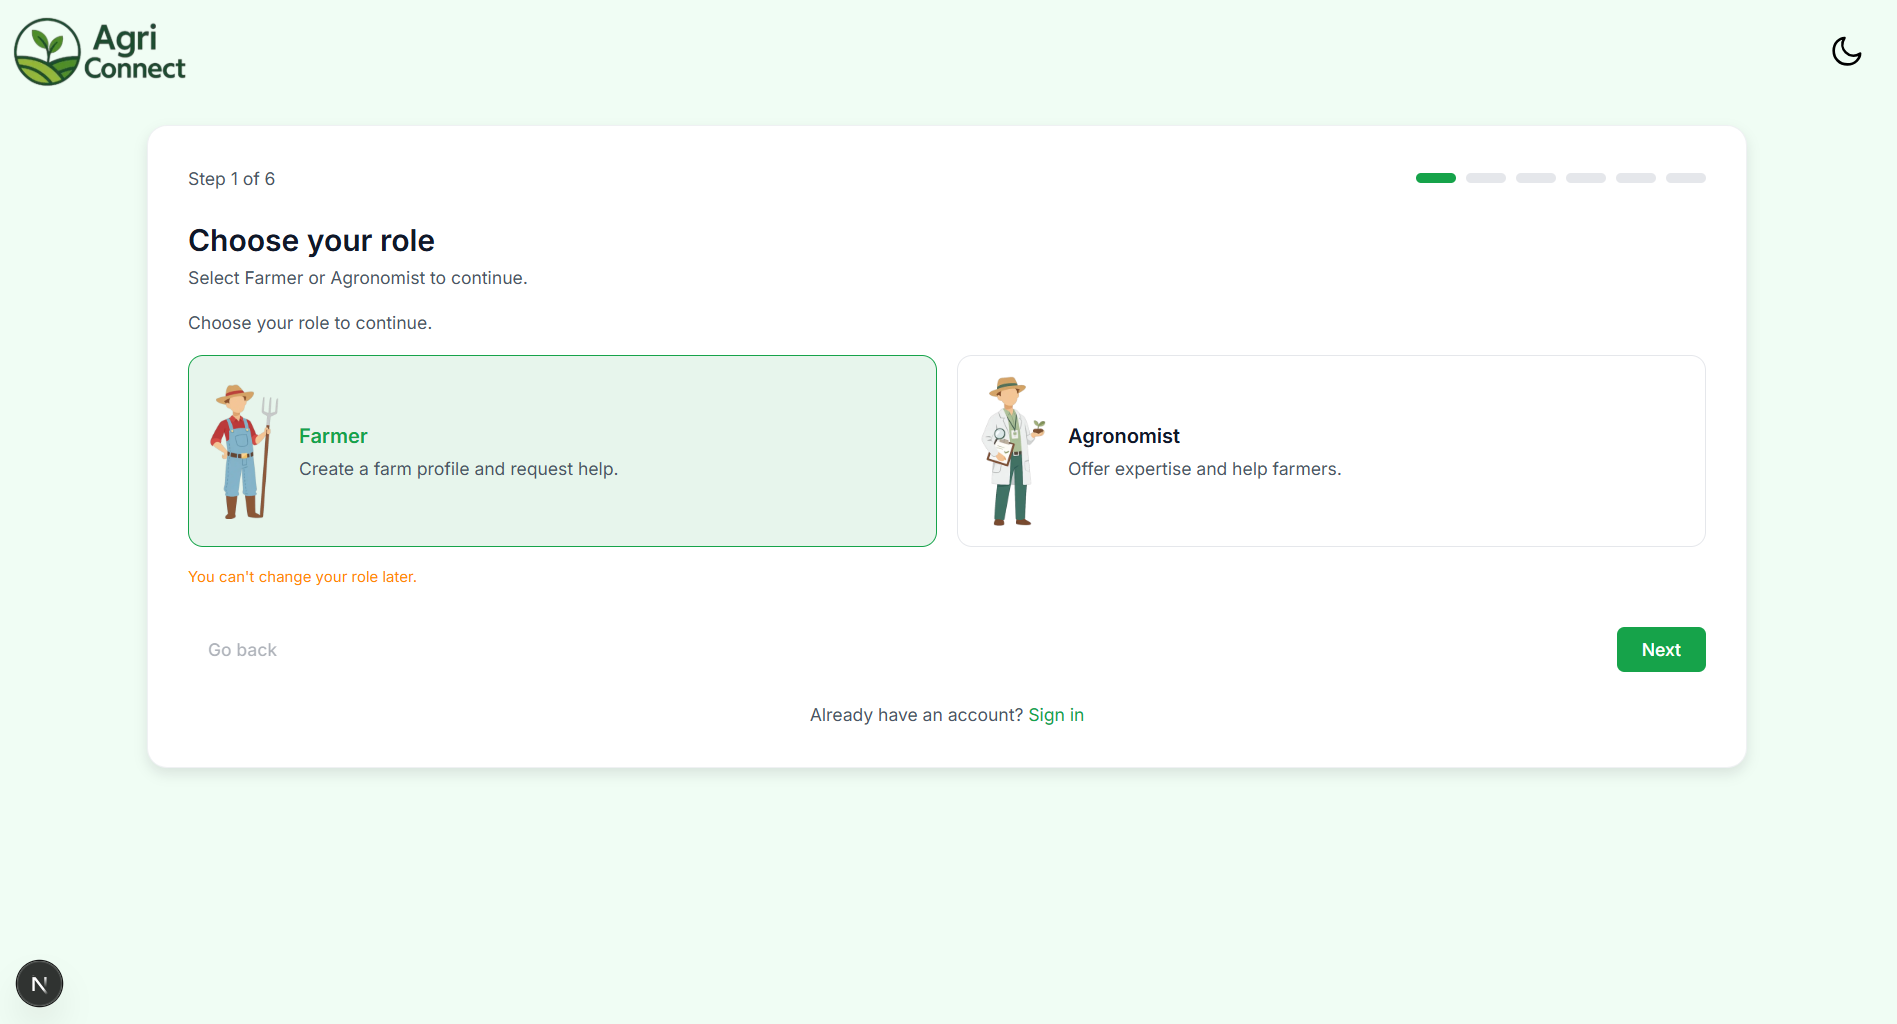
\includegraphics[width=0.8\textwidth]{images/interfaces/visitors/register_page.png}
\caption{Registration page of the AgriConnect web application}
\end{figure}

During registration, users are required to select their role within the platform, either as a farmer or an agronomist. This role determines the functionalities and interfaces that will be accessible after authentication.

Once authenticated, Supabase generates a session containing a JSON Web Token (JWT), which is used to securely communicate with the backend services.

\subsubsection*{Backend Integration and User Identification}

The backend, implemented using Spring Boot, relies on JWT-based authentication to identify users and secure API endpoints. Each request from the frontend includes the access token in the Authorization header.

On the backend side, the user identity is extracted from the JWT token. The system then retrieves the user’s role directly from the database rather than relying solely on token claims. This approach ensures that role information is always up-to-date and consistent.

\subsubsection*{Role-Based Access Control}

Access to different parts of the application is controlled based on user roles. After authentication, the system determines the role of the user and redirects them to the appropriate interface.

For example:
\begin{itemize}
    \item Farmers are redirected to the farmer dashboard.
    \item Agronomists are redirected to the agronomist interface.
\end{itemize}

This redirection is handled at the frontend level by verifying the session and requesting the user profile from the backend. Based on the returned role, the user is directed to the corresponding dashboard.

In addition to frontend checks, backend endpoints are also protected to ensure that users can only access resources permitted by their role. This dual-layer security approach enhances the robustness of the system.

\subsubsection*{Session Management}

Session management is handled by Supabase, which maintains user sessions and provides access tokens for authenticated requests. These tokens are automatically used by the frontend to communicate with the backend services.

\subsubsection*{Admin Access}

The administrator interface is implemented as a separate web application. Although it uses the same authentication mechanism and backend services, it provides a distinct interface dedicated to platform management. Access to this interface is restricted to users with administrative privileges.

Overall, the authentication and authorization system ensures secure, role-based access to the platform while maintaining a seamless user experience.

\subsection{Farmer Interface}

The farmer interface is one of the core components of the AgriConnect web application. It enables farmers to create and manage agricultural cases, interact with agronomists through proposals, and monitor the progress of their requests.

\subsubsection*{Dashboard}

The farmer dashboard serves as the main entry point after authentication. It provides an overview of the farmer’s activity through key statistics and quick access to important features.

The dashboard displays information such as the total number of cases, open cases, assigned cases, and closed cases. It also includes shortcuts that allow users to quickly perform actions such as creating a new case or accessing their profile.

\begin{figure}[H]
\centering
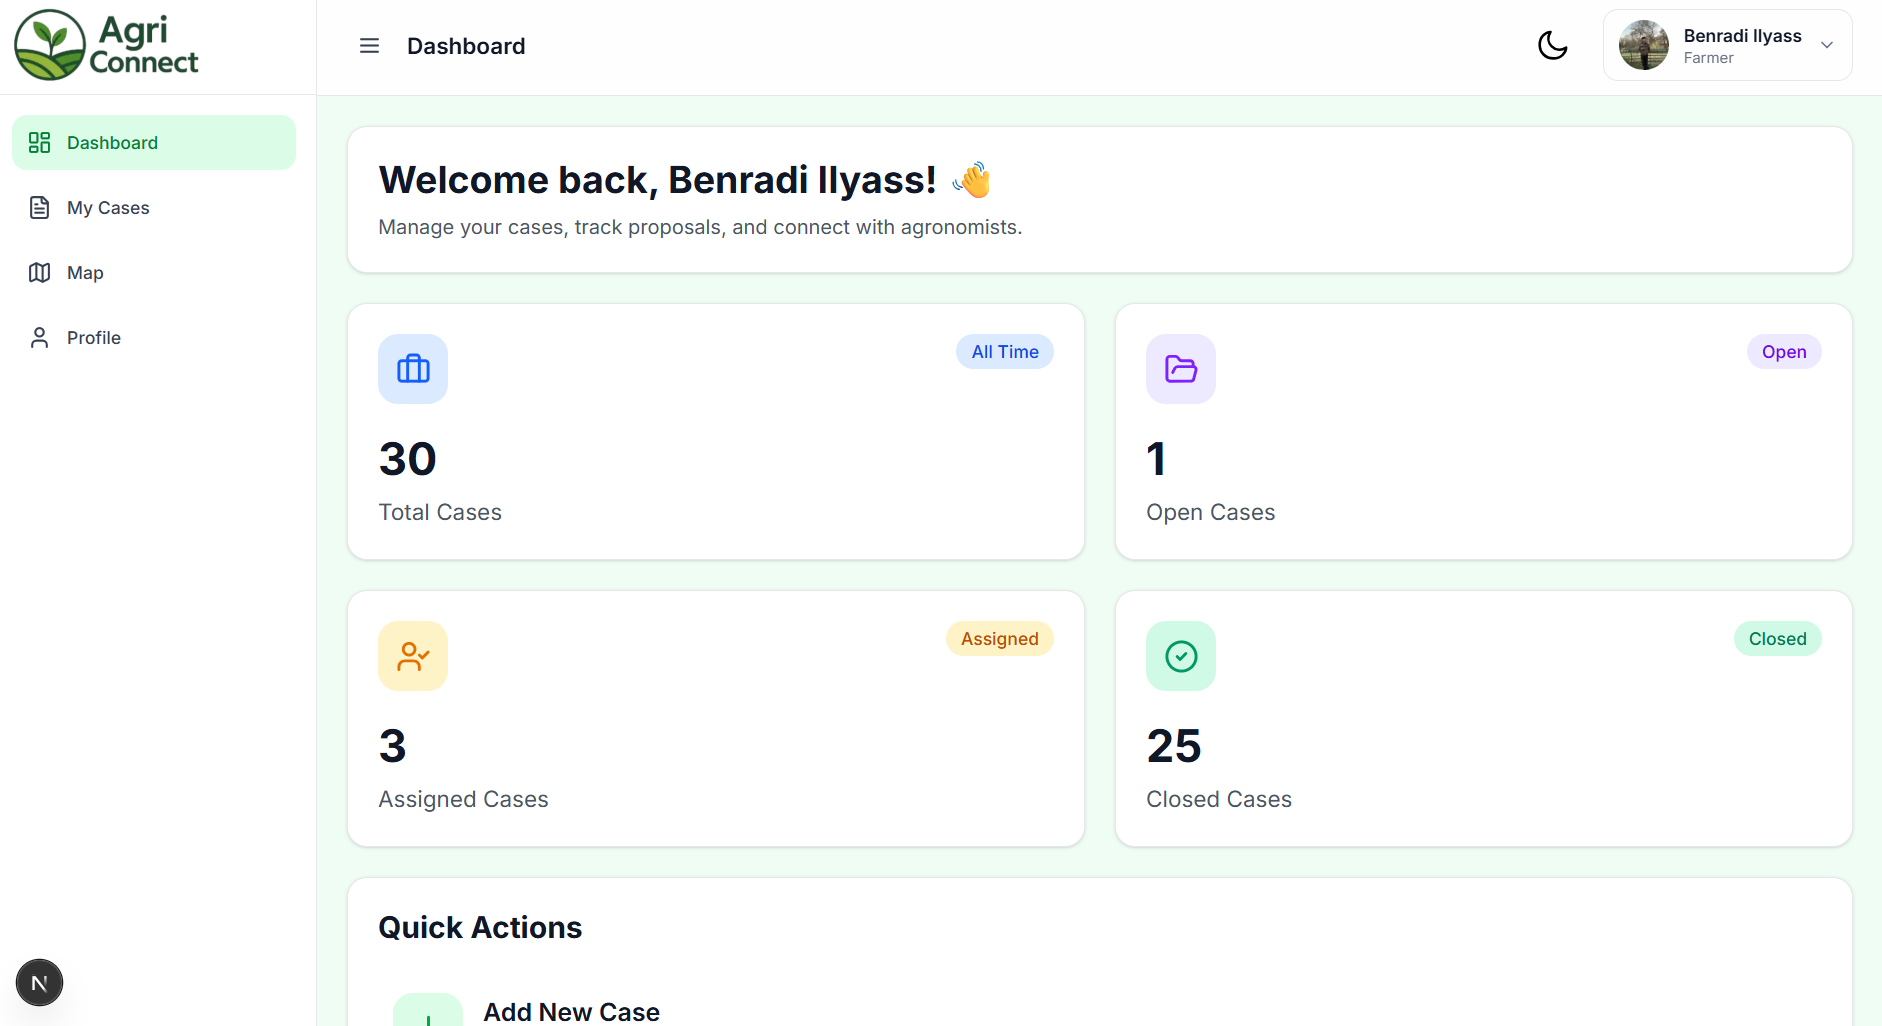
\includegraphics[width=0.9\textwidth]{images/interfaces/farmer/farmer_dashboard.png}
\caption{Farmer dashboard showing statistics and quick actions}
\end{figure}

\subsubsection*{Case Creation}

Farmers can create new agricultural cases manually through a dedicated form. The case creation process includes several fields such as the title, summary, priority level, and the ability to upload multiple images.

The support for multiple image uploads allows farmers to provide more context about their agricultural issues, improving the quality of analysis and responses.

\begin{figure}[H]
\centering
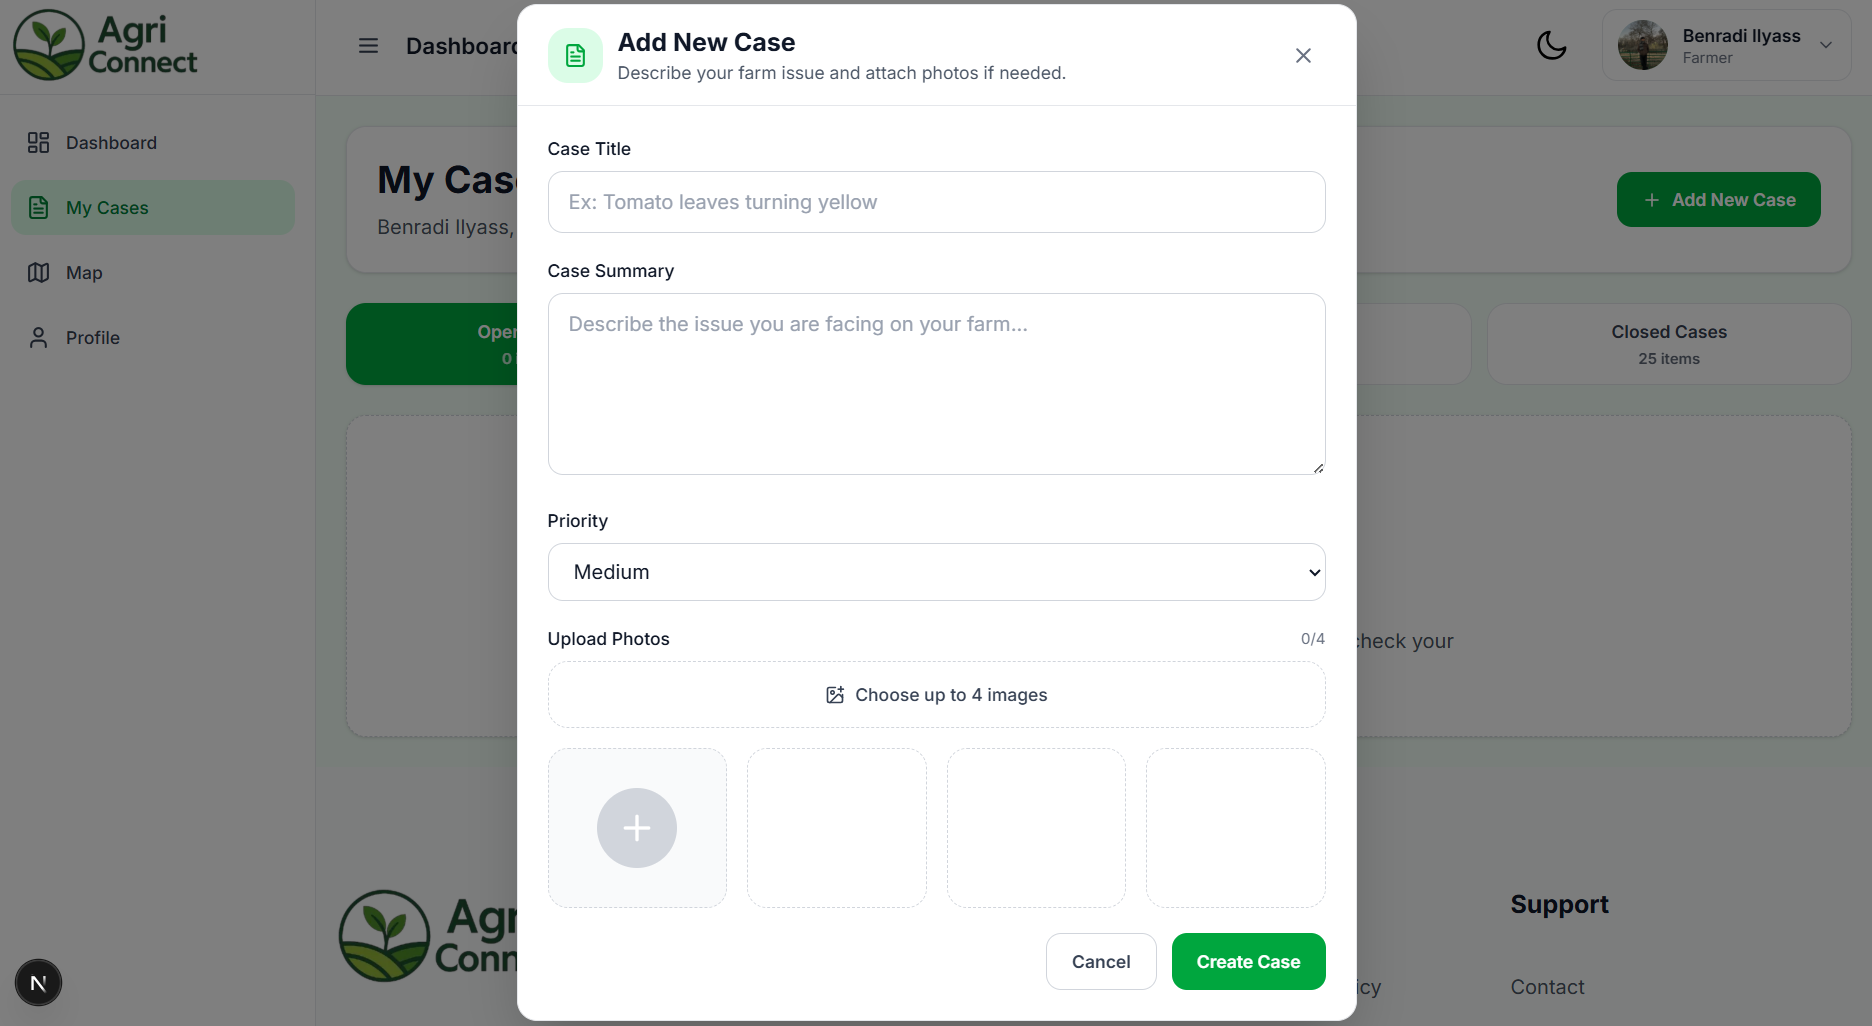
\includegraphics[width=0.9\textwidth]{images/interfaces/farmer/create_case.png}
\caption{Case creation interface with multi-image upload}
\end{figure}

\subsubsection*{Case Management}

The ``My Cases'' page allows farmers to manage all their submitted cases. The interface is organized into multiple sections based on the status of each case: open, in progress, resolved, and closed.

Each case is represented by a card containing key information such as the title, summary, status, priority, type (manual or generated via WhatsApp), number of uploaded images, and creation date.

\begin{figure}[H]
\centering
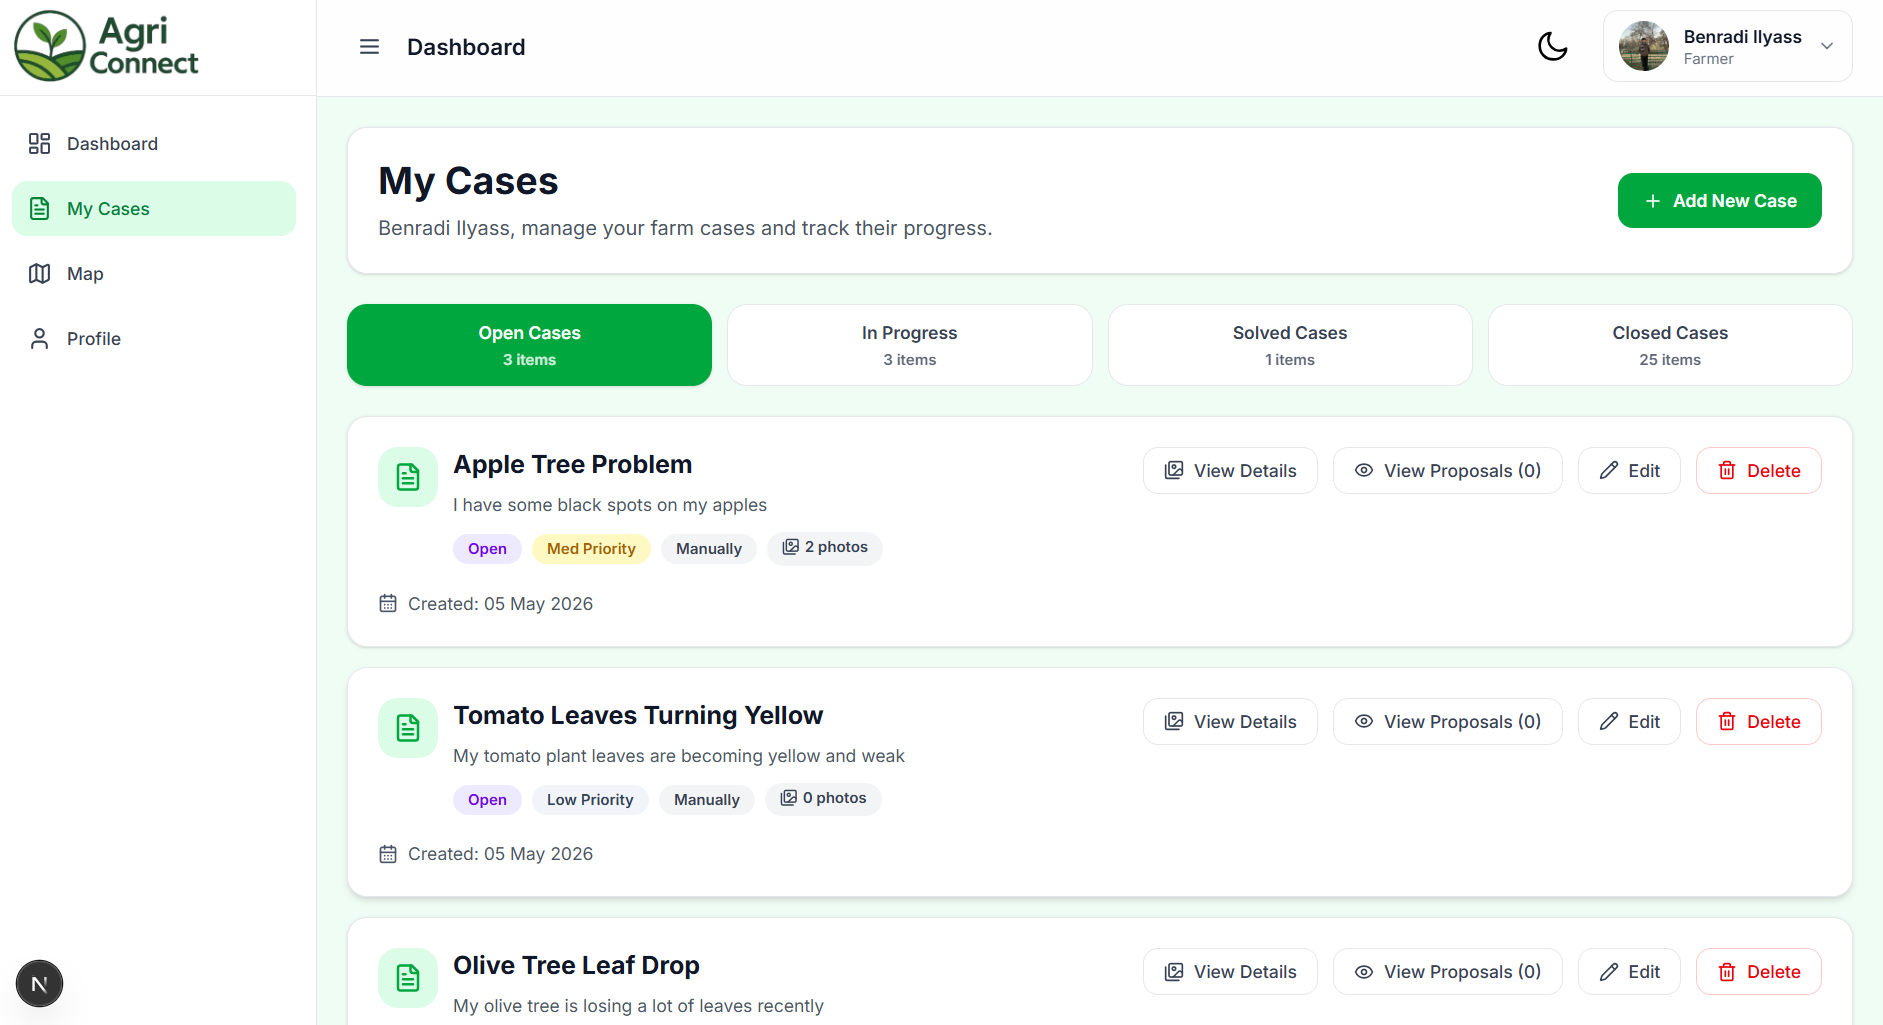
\includegraphics[width=0.9\textwidth]{images/interfaces/farmer/my_cases.png}
\caption{Farmer case management interface organized by status}
\end{figure}

Farmers can perform several actions on each case:

\begin{itemize}
    \item \textbf{View Details:} Displays detailed information about the case, including uploaded images, in a modal interface.
    \item \textbf{View Proposals:} Opens a modal showing proposals submitted by agronomists.
    \item \textbf{Edit and Delete:} Allows modification or deletion of a case, but only when the case is still in the open state.
\end{itemize}

\subsubsection*{Proposal Interaction}

The interaction between farmers and agronomists is handled through a proposal system. Agronomists can submit proposals for open cases, and farmers can review them through the interface.

Farmers have the ability to accept or reject proposals. Once a proposal is accepted, the corresponding agronomist becomes responsible for the case, and its status is updated accordingly.

\begin{figure}[H]
\centering
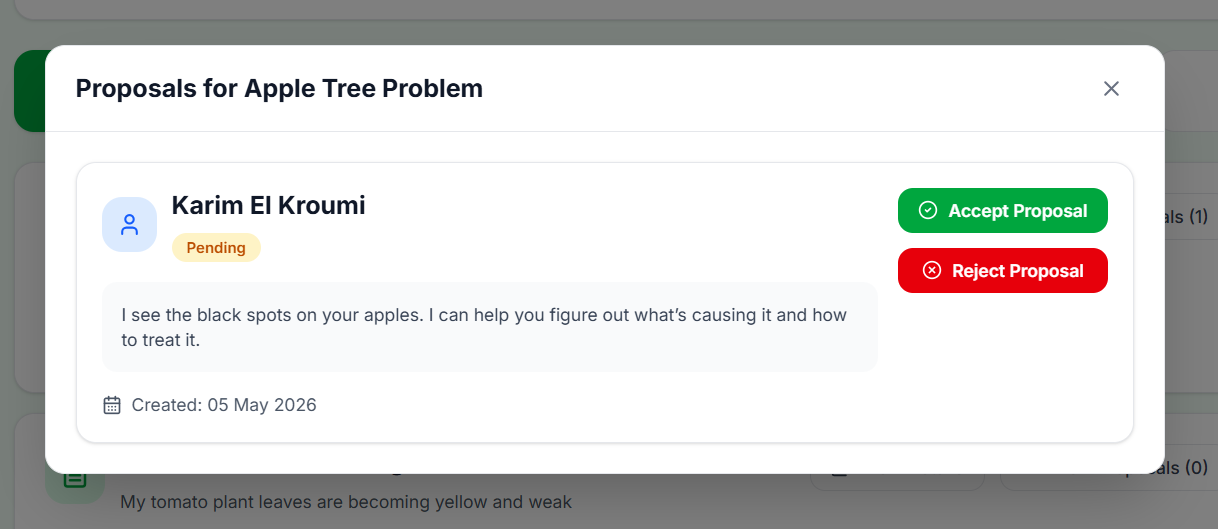
\includegraphics[width=0.9\textwidth]{images/interfaces/farmer/proposals_modal.png}
\caption{Proposals interface allowing farmers to review and accept agronomist offers}
\end{figure}

Overall, the farmer interface provides a structured and user-friendly environment that allows farmers to efficiently manage their agricultural issues, track their evolution, and collaborate with agronomists.

\subsection{Agronomist Interface}

The agronomist interface is designed to enable experts to analyze agricultural cases, provide recommendations, and interact with farmers through a structured proposal system. It provides tools for browsing available cases, managing proposals, and following the progress of assigned cases.

\subsubsection*{Dashboard}

The agronomist dashboard serves as the main entry point after authentication. It provides an overview of the agronomist’s activity through key statistics and quick navigation options.

The dashboard displays information such as the total number of assigned cases, pending cases, cases in progress, and resolved cases. It also includes shortcuts that allow users to quickly access important sections such as pending cases and assigned cases.

\begin{figure}[H]
\centering
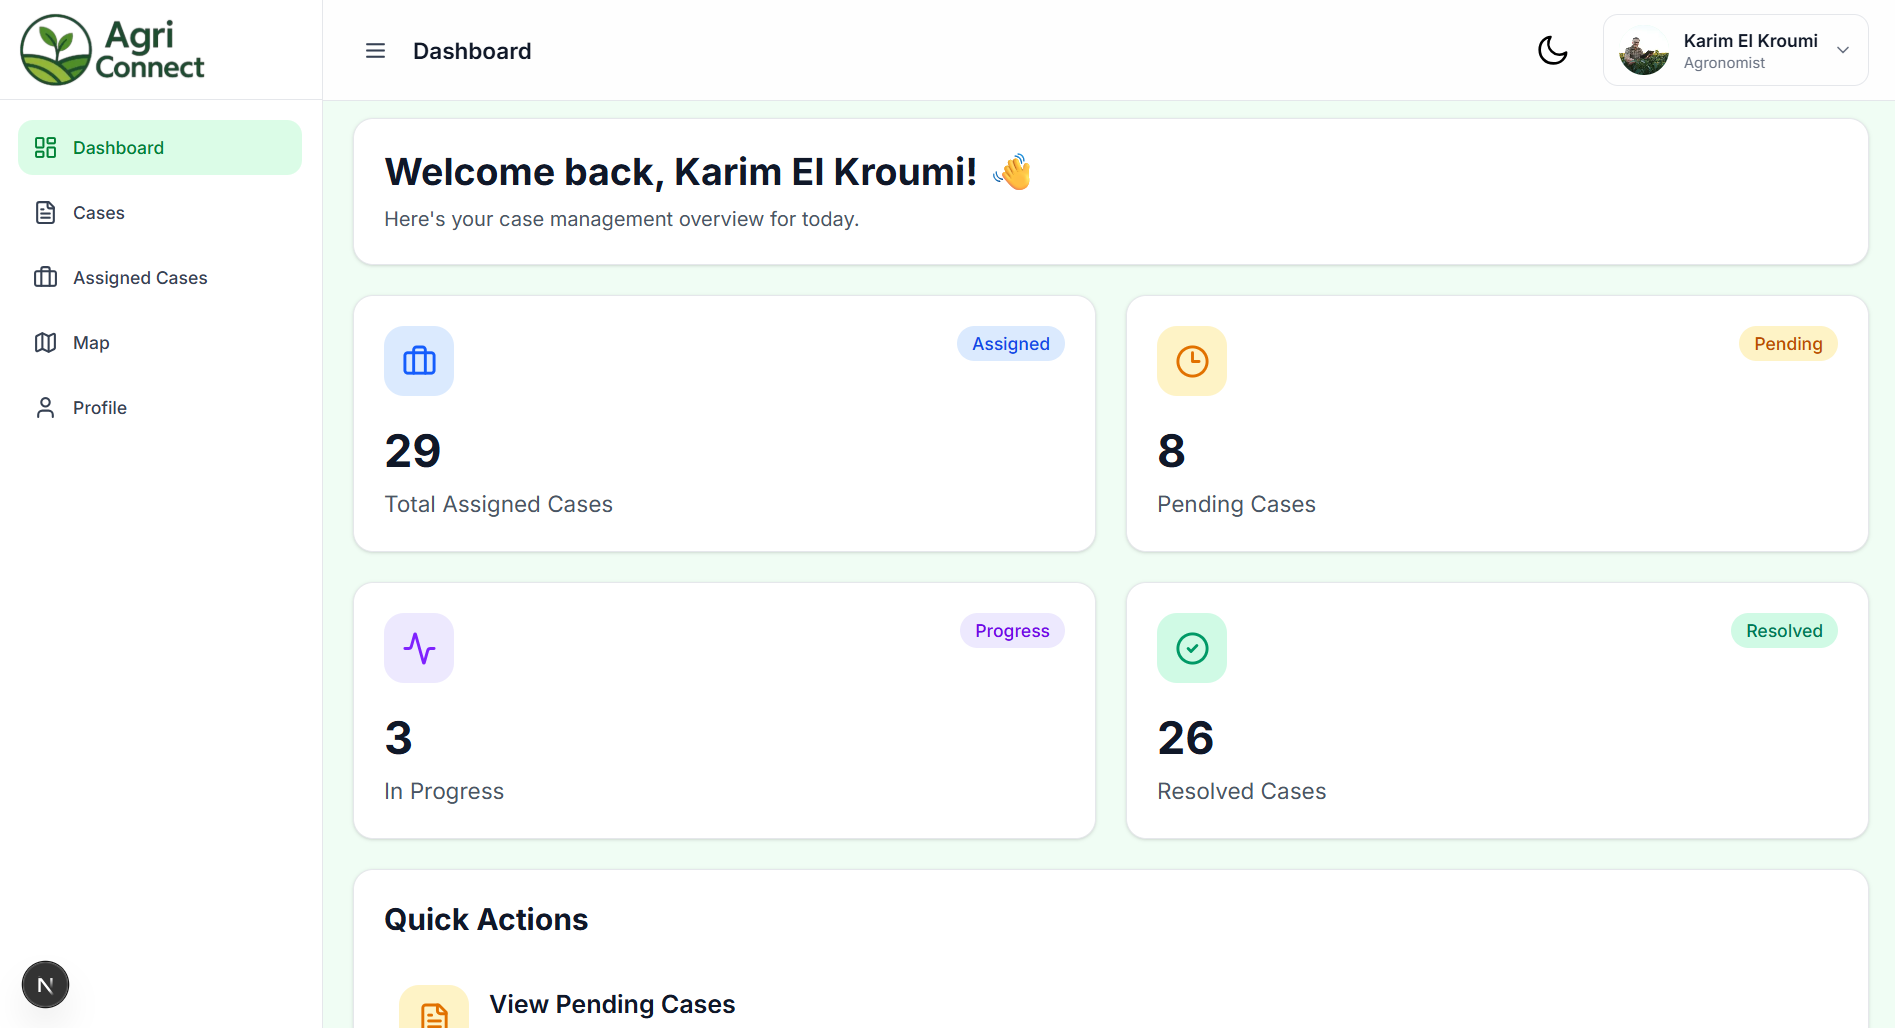
\includegraphics[width=0.9\textwidth]{images/interfaces/agronomists/agronomist_dashboard.png}
\caption{Agronomist dashboard displaying activity statistics and shortcuts}
\end{figure}

\subsubsection*{Case Exploration and Proposal Creation}

Agronomists can browse open cases through the ``Cases'' page. This section contains all cases that have not yet been assigned to any agronomist.

Each case is presented using a card-based interface similar to the farmer view, displaying key information such as title, summary, status, priority, and associated images. However, agronomists are provided with different actions tailored to their role.

\begin{figure}[H]
\centering
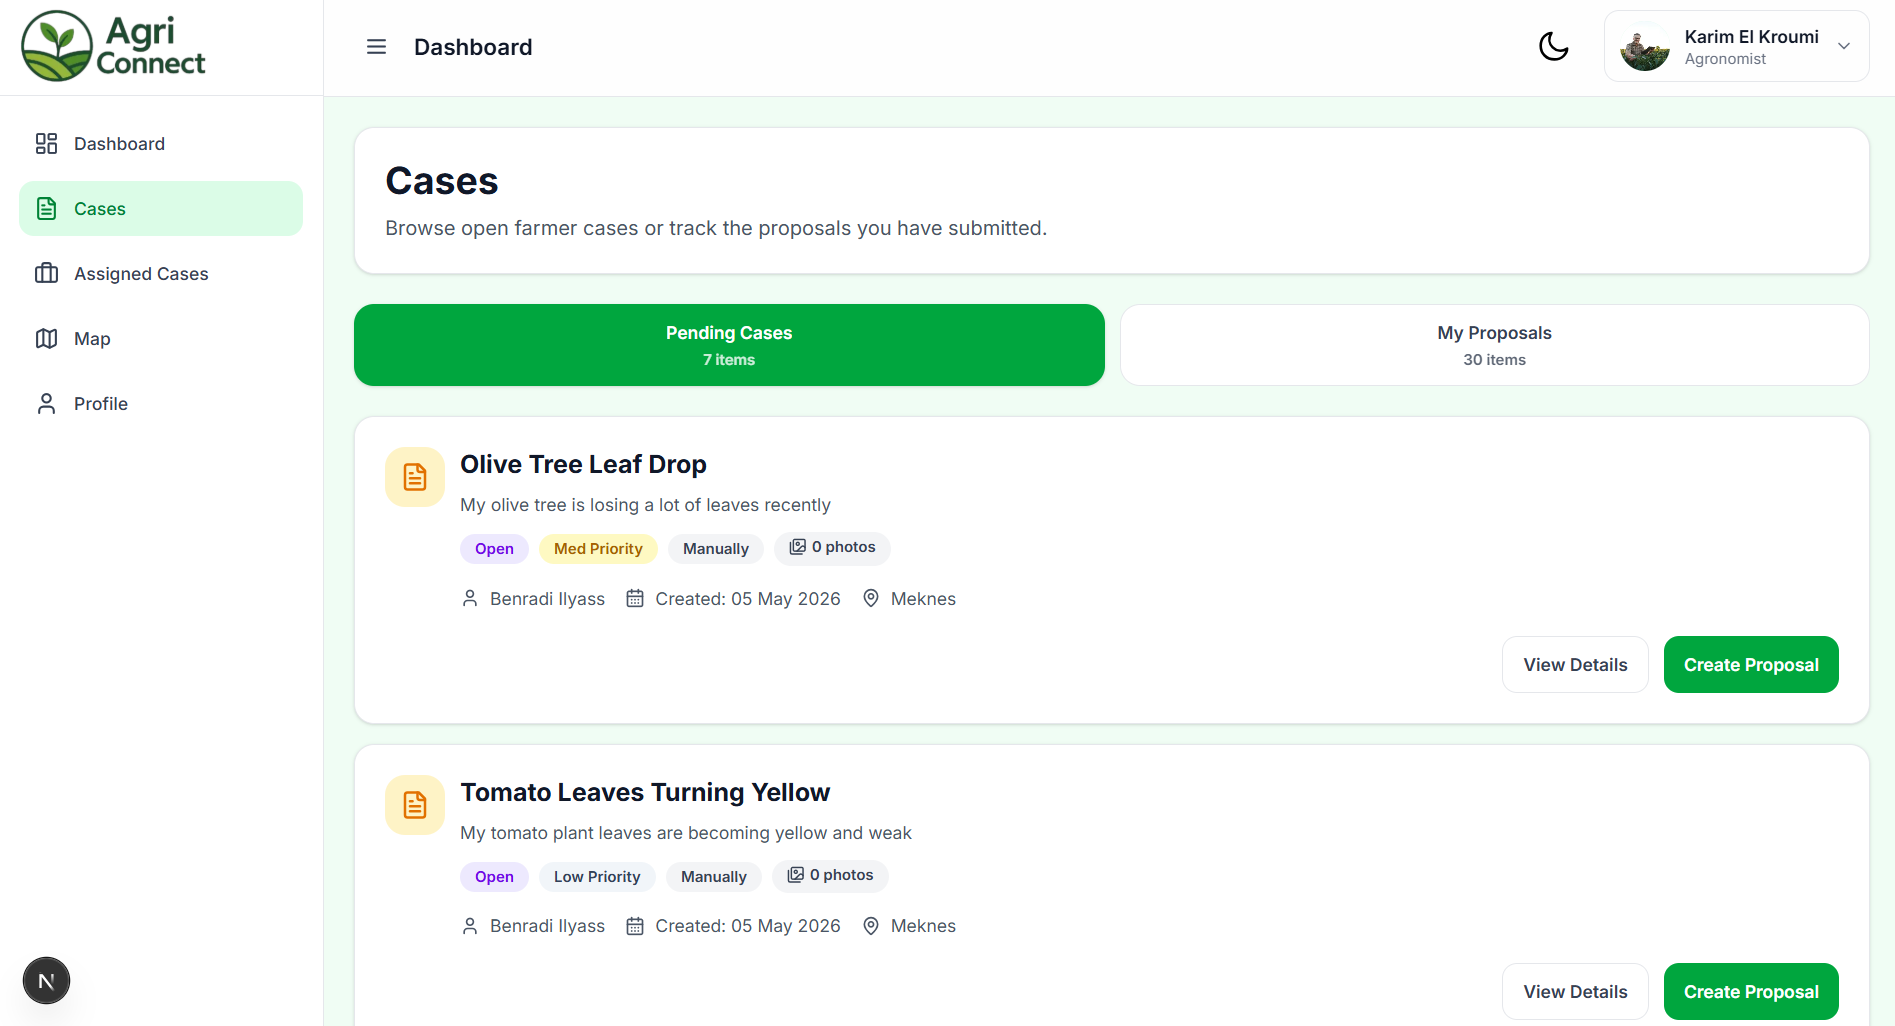
\includegraphics[width=0.9\textwidth]{images/interfaces/agronomists/pending_cases.png}
\caption{Pending cases available for agronomists}
\end{figure}

For each case, agronomists can:

\begin{itemize}
    \item \textbf{View Details:} Access complete case information and uploaded images.
    \item \textbf{Create Proposal:} Submit a proposal to assist the farmer by providing a message describing the recommended solution or approach.
\end{itemize}

\subsubsection*{Proposal Management}

The ``My Proposals'' section allows agronomists to manage all submitted proposals. This section is organized into three categories based on proposal status:

\begin{itemize}
    \item \textbf{Pending:} proposals awaiting farmer decision.
    \item \textbf{Accepted:} proposals that have been approved by farmers.
    \item \textbf{Rejected:} proposals that have been declined.
\end{itemize}

\begin{figure}[H]
\centering
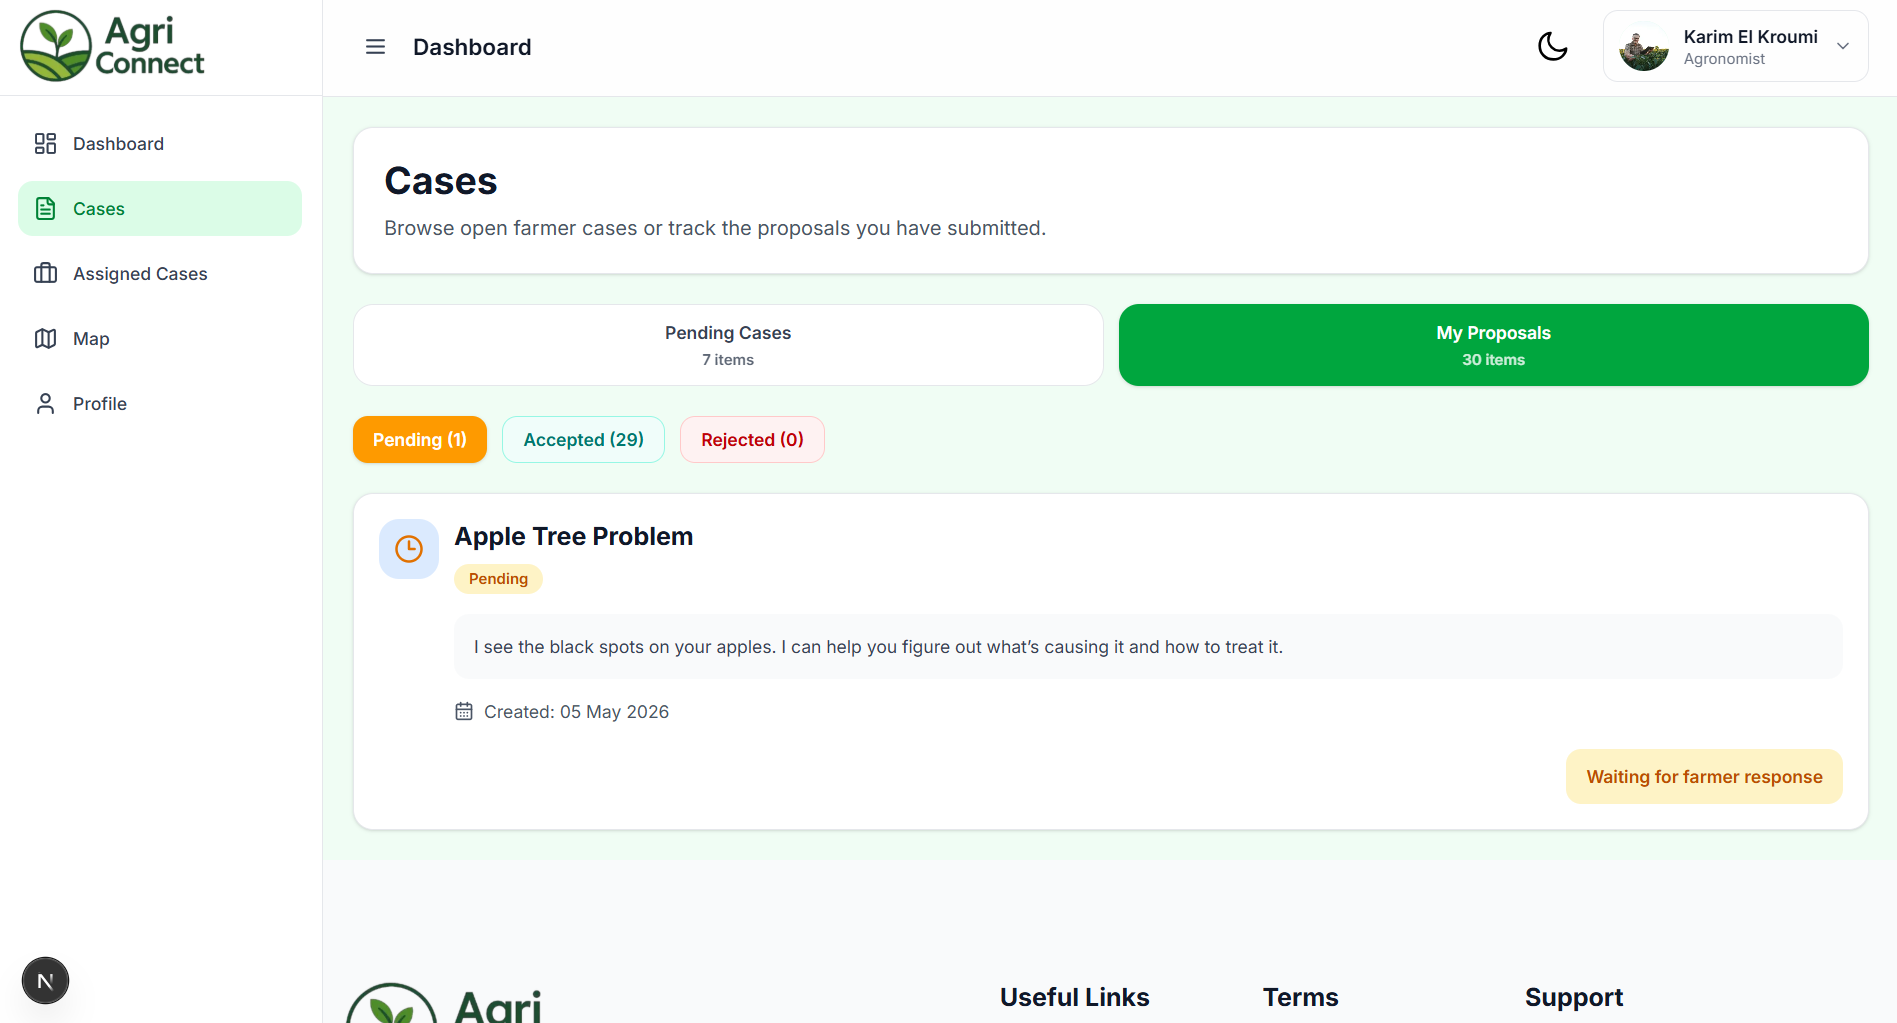
\includegraphics[width=0.9\textwidth]{images/interfaces/agronomists/my_proposals.png}
\caption{Agronomist proposal management interface}
\end{figure}

\subsubsection*{Assigned Case Management}

Once a proposal is accepted, the agronomist becomes responsible for the case. The case is then moved to the ``Assigned Cases'' section and its status is updated to ``in progress''.

This section is divided into three categories:

\begin{itemize}
    \item \textbf{In Progress:} cases currently being handled by the agronomist.
    \item \textbf{Resolved:} cases marked as resolved by the agronomist but not yet closed.
    \item \textbf{Closed:} cases that have been fully completed after farmer validation.
\end{itemize}

\begin{figure}[H]
\centering
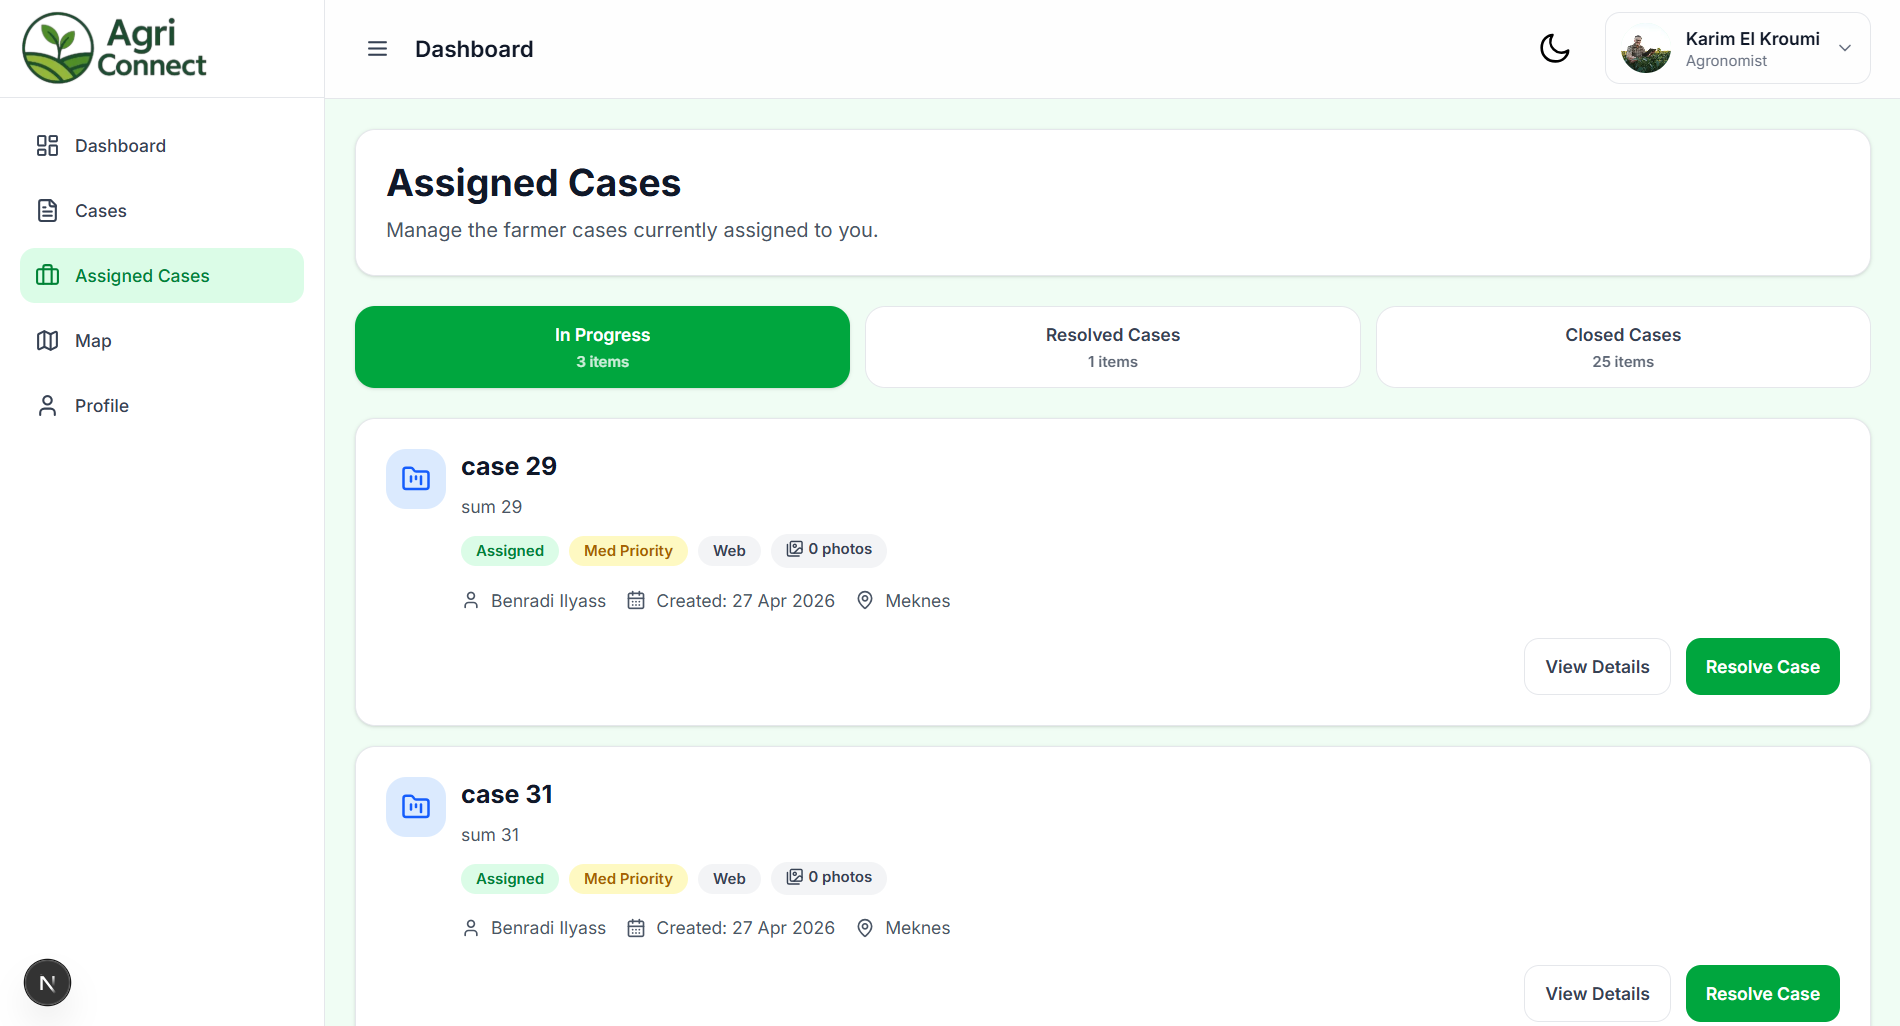
\includegraphics[width=0.9\textwidth]{images/interfaces/agronomists/assigned_cases.png}
\caption{Assigned cases managed by the agronomist}
\end{figure}

In this workflow, the agronomist is responsible for analyzing the case and providing a solution. Once the issue is addressed, the agronomist can mark the case as resolved. The final closure of the case depends on the farmer’s feedback.

Overall, the agronomist interface provides a structured environment that allows experts to efficiently manage agricultural cases, interact with farmers through proposals, and track the progress of their interventions.

\subsection{Shared Interfaces}

In addition to role-specific interfaces, the AgriConnect web application provides a set of shared interfaces accessible to both farmers and agronomists. These interfaces promote interaction, visibility, and profile management across the platform.

\subsubsection*{Interactive Map}

The map interface provides a geographical visualization of users across Morocco. It is implemented as an interactive map displaying all registered users based on their location.

Each user is represented by a marker, with a color indicating their role:
\begin{itemize}
    \item Orange markers represent farmers.
    \item Blue markers represent agronomists.
    \item A green marker represents the currently authenticated user.
\end{itemize}

The location data is stored in a dedicated database table containing geographical attributes such as city, region, commune, latitude, and longitude.

The map supports user interaction in two forms:

\begin{itemize}
    \item \textbf{Hover Interaction:} displays a quick preview including the user’s avatar, name, role, phone number, and location.
    \item \textbf{Click Interaction:} opens a detailed profile card with extended information about the selected user.
\end{itemize}

In addition, the map includes a search functionality that allows users to find other users by name, facilitating discovery and interaction within the platform.

\begin{figure}[H]
\centering
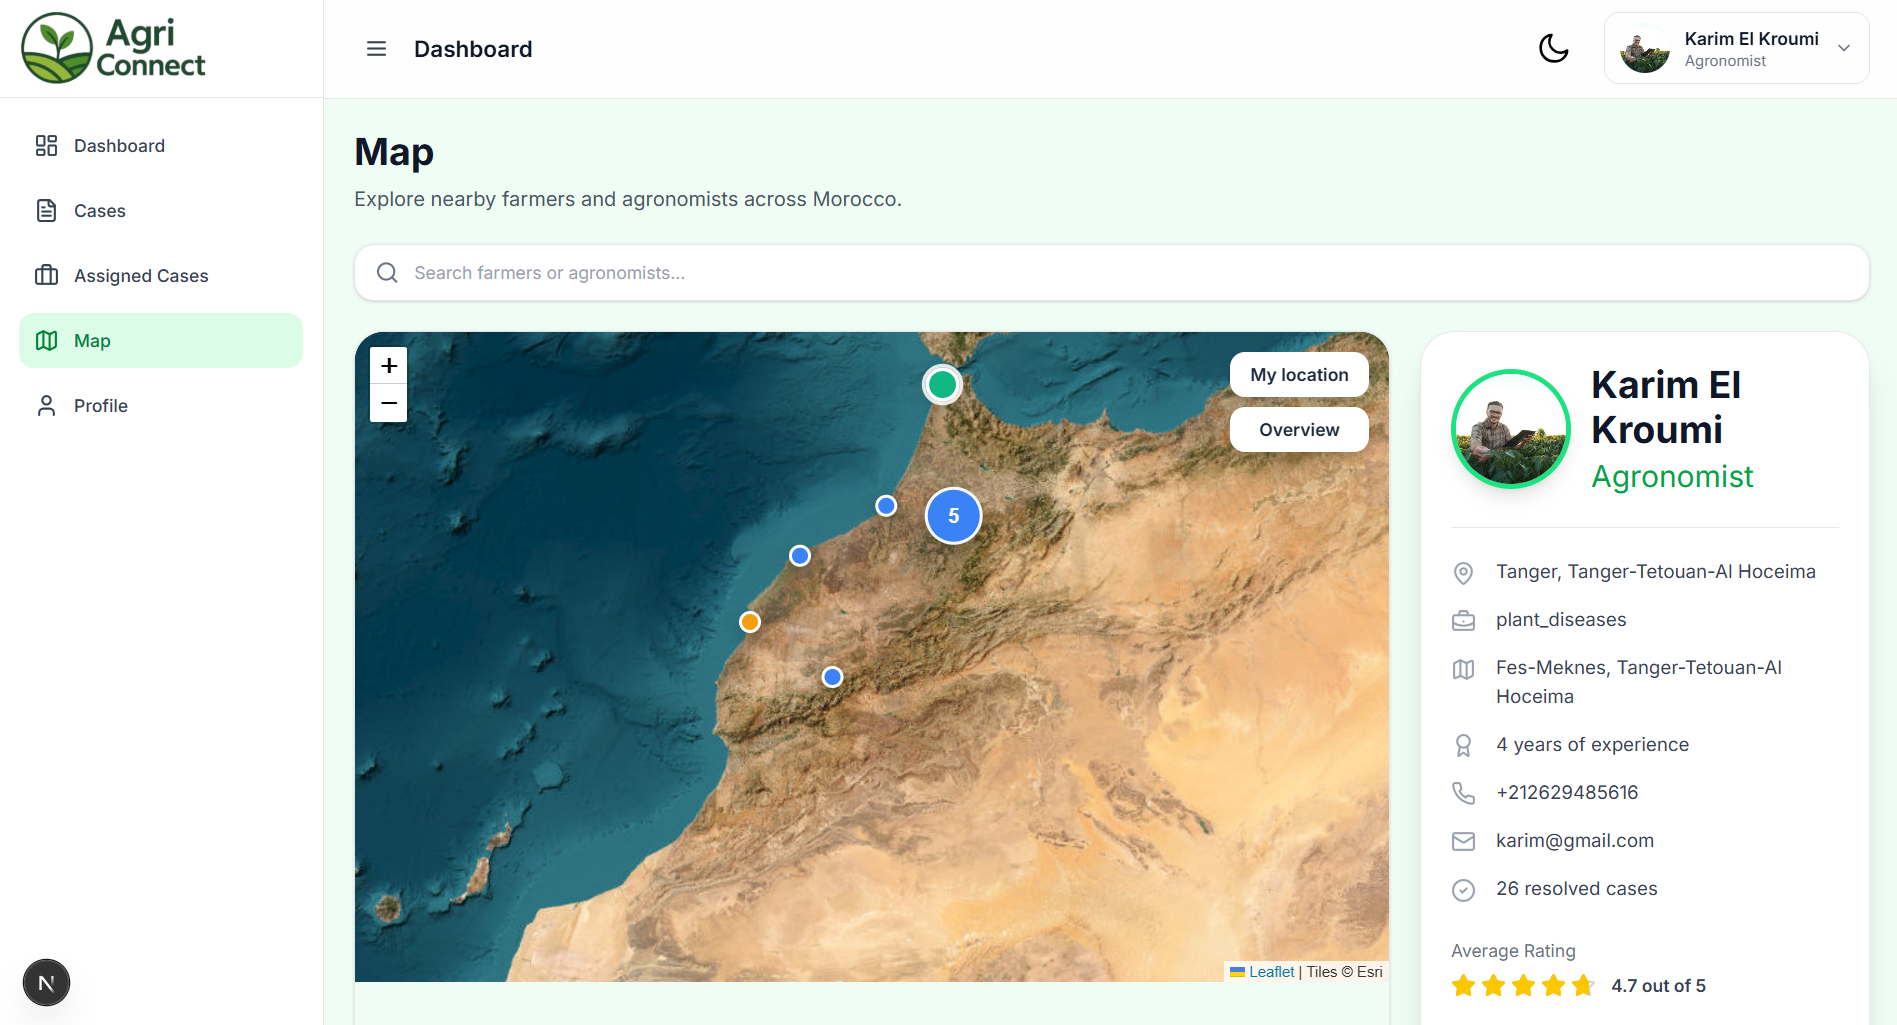
\includegraphics[width=0.9\textwidth]{images/interfaces/shared/map_page.png}
\caption{Interactive map displaying users across Morocco}
\end{figure}

\subsubsection*{Profile Page}

The profile interface allows authenticated users to view and manage their personal information. Each user has access only to their own profile, ensuring data privacy and security.

Users can update various fields such as their avatar, personal information, contact details, and domain-specific attributes. The avatar is stored in Supabase Storage and linked to the user profile.

The structure of the profile page varies depending on the user’s role. Farmers and agronomists have different sets of attributes reflecting their specific activities and expertise.

\begin{figure}[H]
\centering
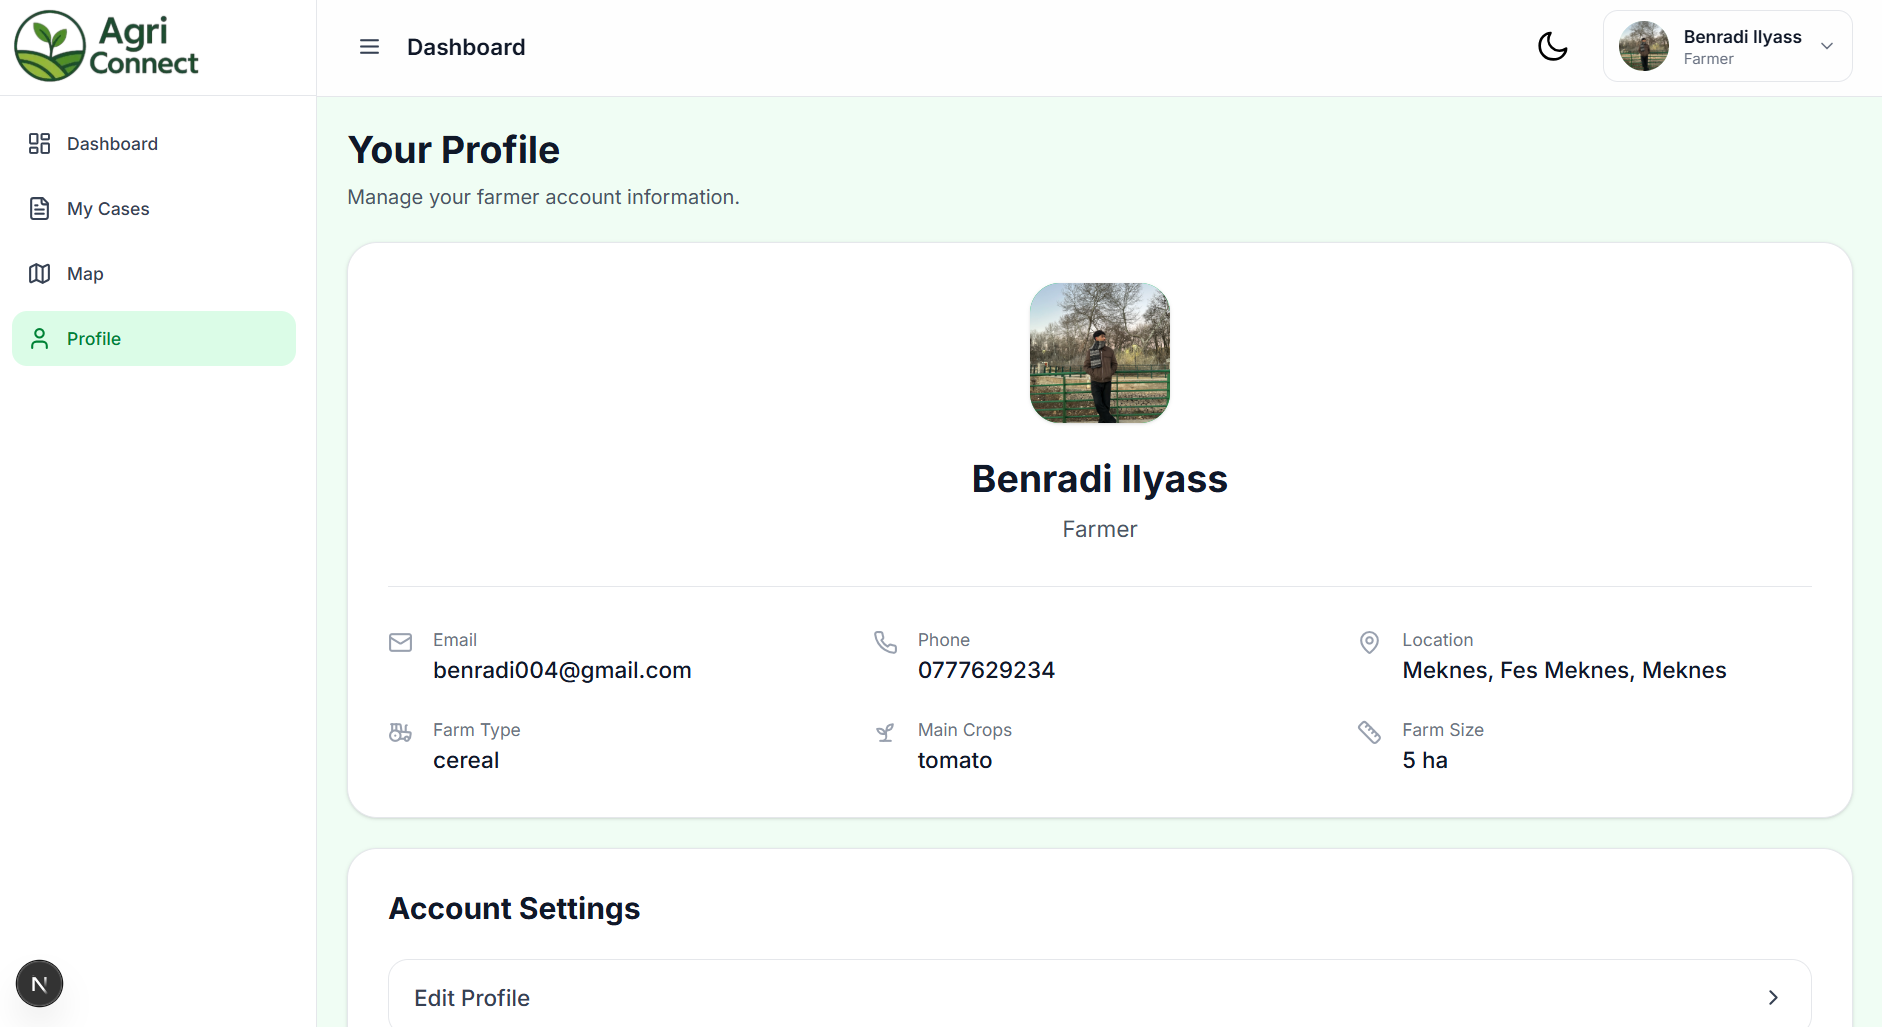
\includegraphics[width=0.6\textwidth]{images/interfaces/shared/farmer_profile.png}
\caption{Example of farmer profile interface}
\end{figure}

\begin{figure}[H]
\centering
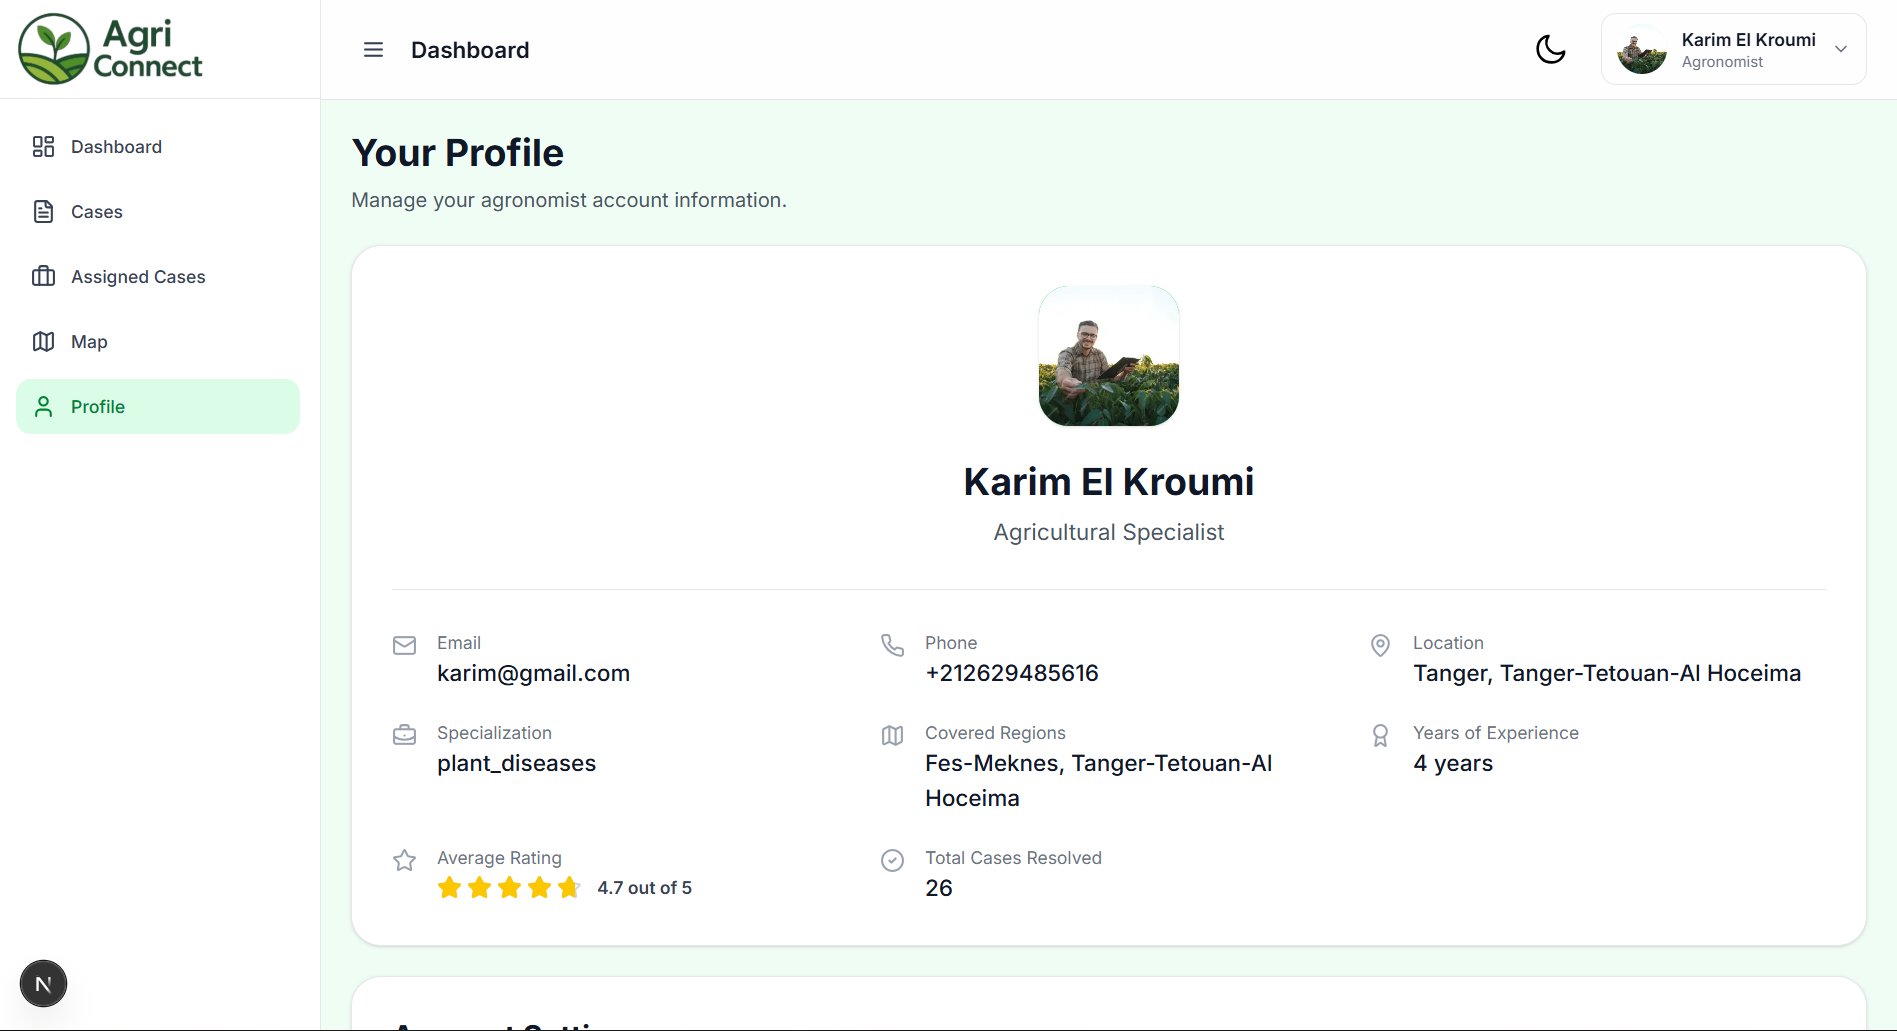
\includegraphics[width=0.6\textwidth]{images/interfaces/shared/agronomist_profile.png}
\caption{Example of agronomist profile interface}
\end{figure}

Overall, these shared interfaces enhance the platform by providing a unified space for user interaction, geographical visualization, and personalized profile management, while maintaining consistency across different user roles.


\subsection{Admin Dashboard}

The admin dashboard is implemented as a separate web application dedicated to platform supervision and management. It provides administrators with full control over users, cases, proposals, and feedback, ensuring proper system operation.

\subsubsection*{Admin Authentication}

Access to the admin interface is restricted through a dedicated login page. Although it relies on the same authentication mechanism as the main application, it is deployed as a separate interface to ensure better separation of concerns and enhanced security.

Administrators must authenticate using their credentials before accessing the dashboard functionalities.

\begin{figure}[H]
\centering

\includegraphics[width=0.7\textwidth]{images/interfaces/admin/admin_login.png}
\caption{Admin login interface}
\end{figure}

\subsubsection*{Dashboard Overview}

After authentication, administrators are redirected to the main dashboard, which provides a global view of platform activity through key statistics and visualizations.

The dashboard displays metrics such as the total number of users, farmers, agronomists, total cases, and open cases. It also includes a circular chart representing the distribution of cases based on their status (open, assigned, resolved, and closed), as well as a list of recently updated cases.

\begin{figure}[H]
\centering
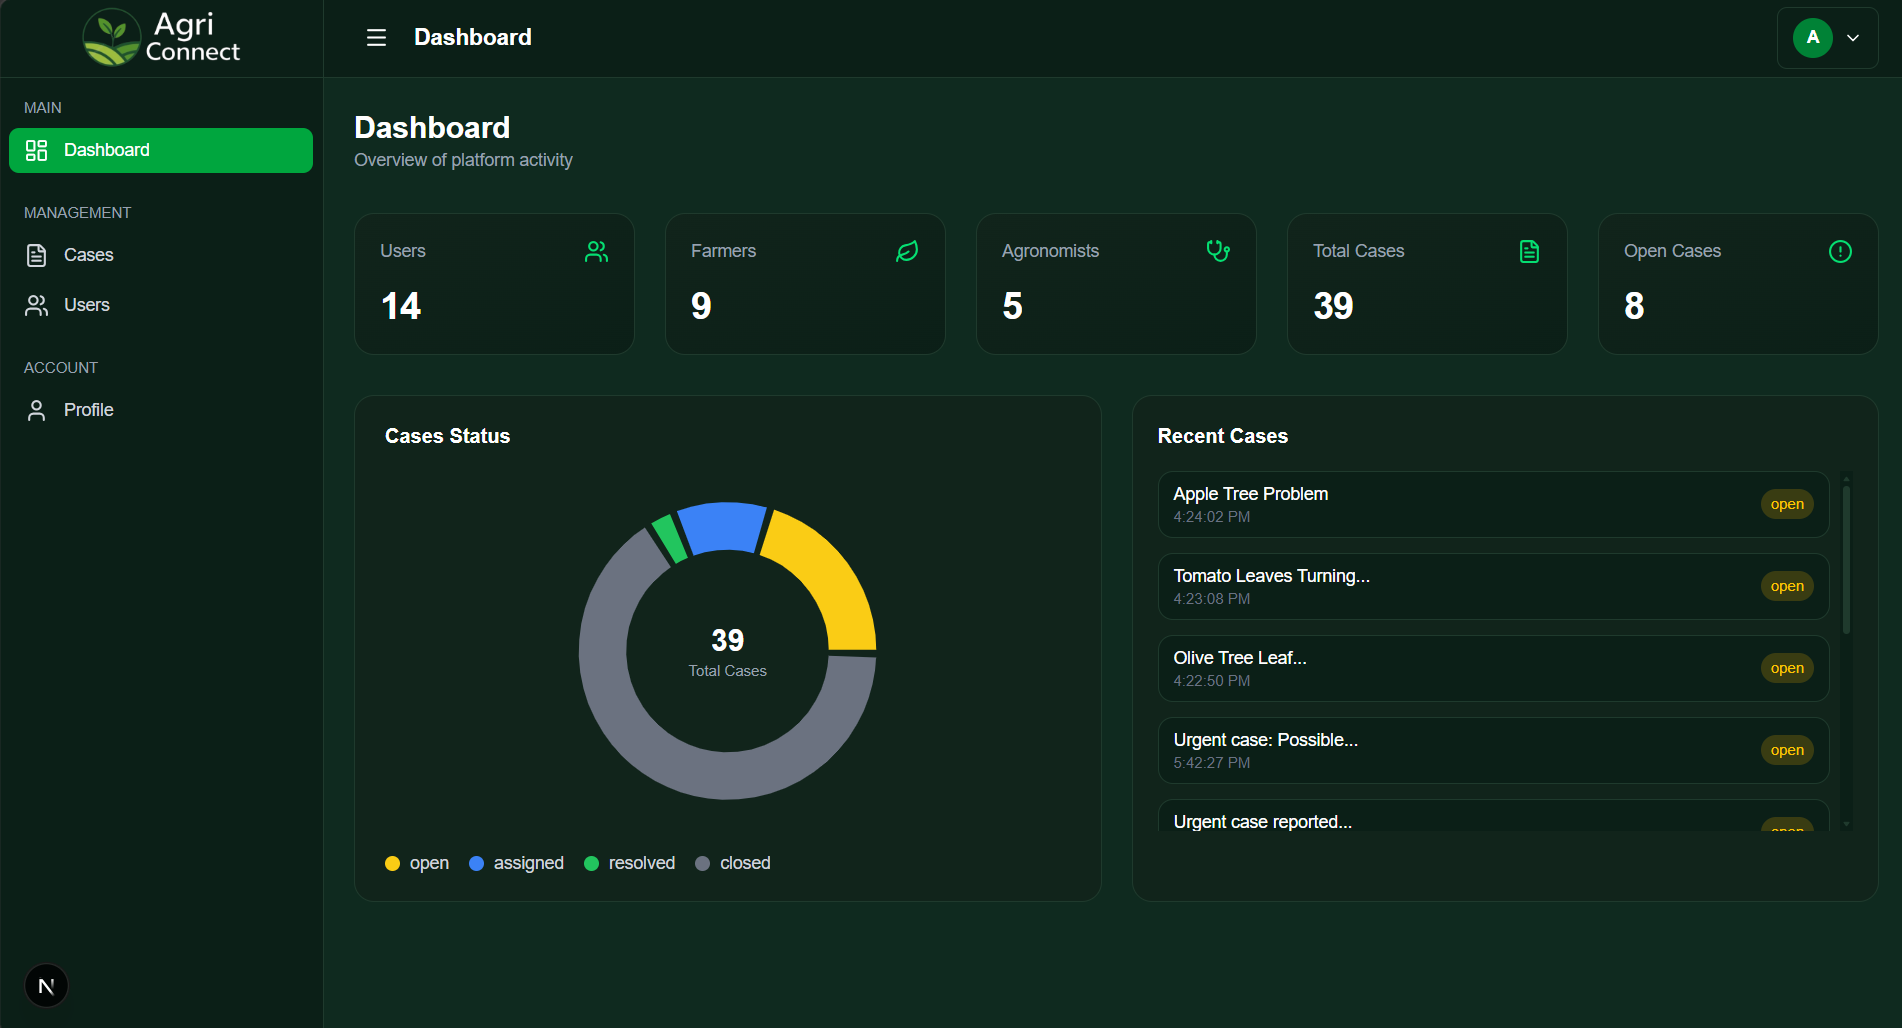
\includegraphics[width=0.9\textwidth]{images/interfaces/admin/admin_dashboard.png}
\caption{Admin dashboard showing global statistics and recent activity}
\end{figure}

\subsubsection*{Case Management}

The admin interface provides full access to all cases in the system. Cases are organized into four sections based on their status: open, assigned, resolved, and closed.

Each case is displayed using a card interface similar to the farmer view, but with extended administrative capabilities. Administrators can edit or delete cases regardless of their status.

\begin{figure}[H]
\centering
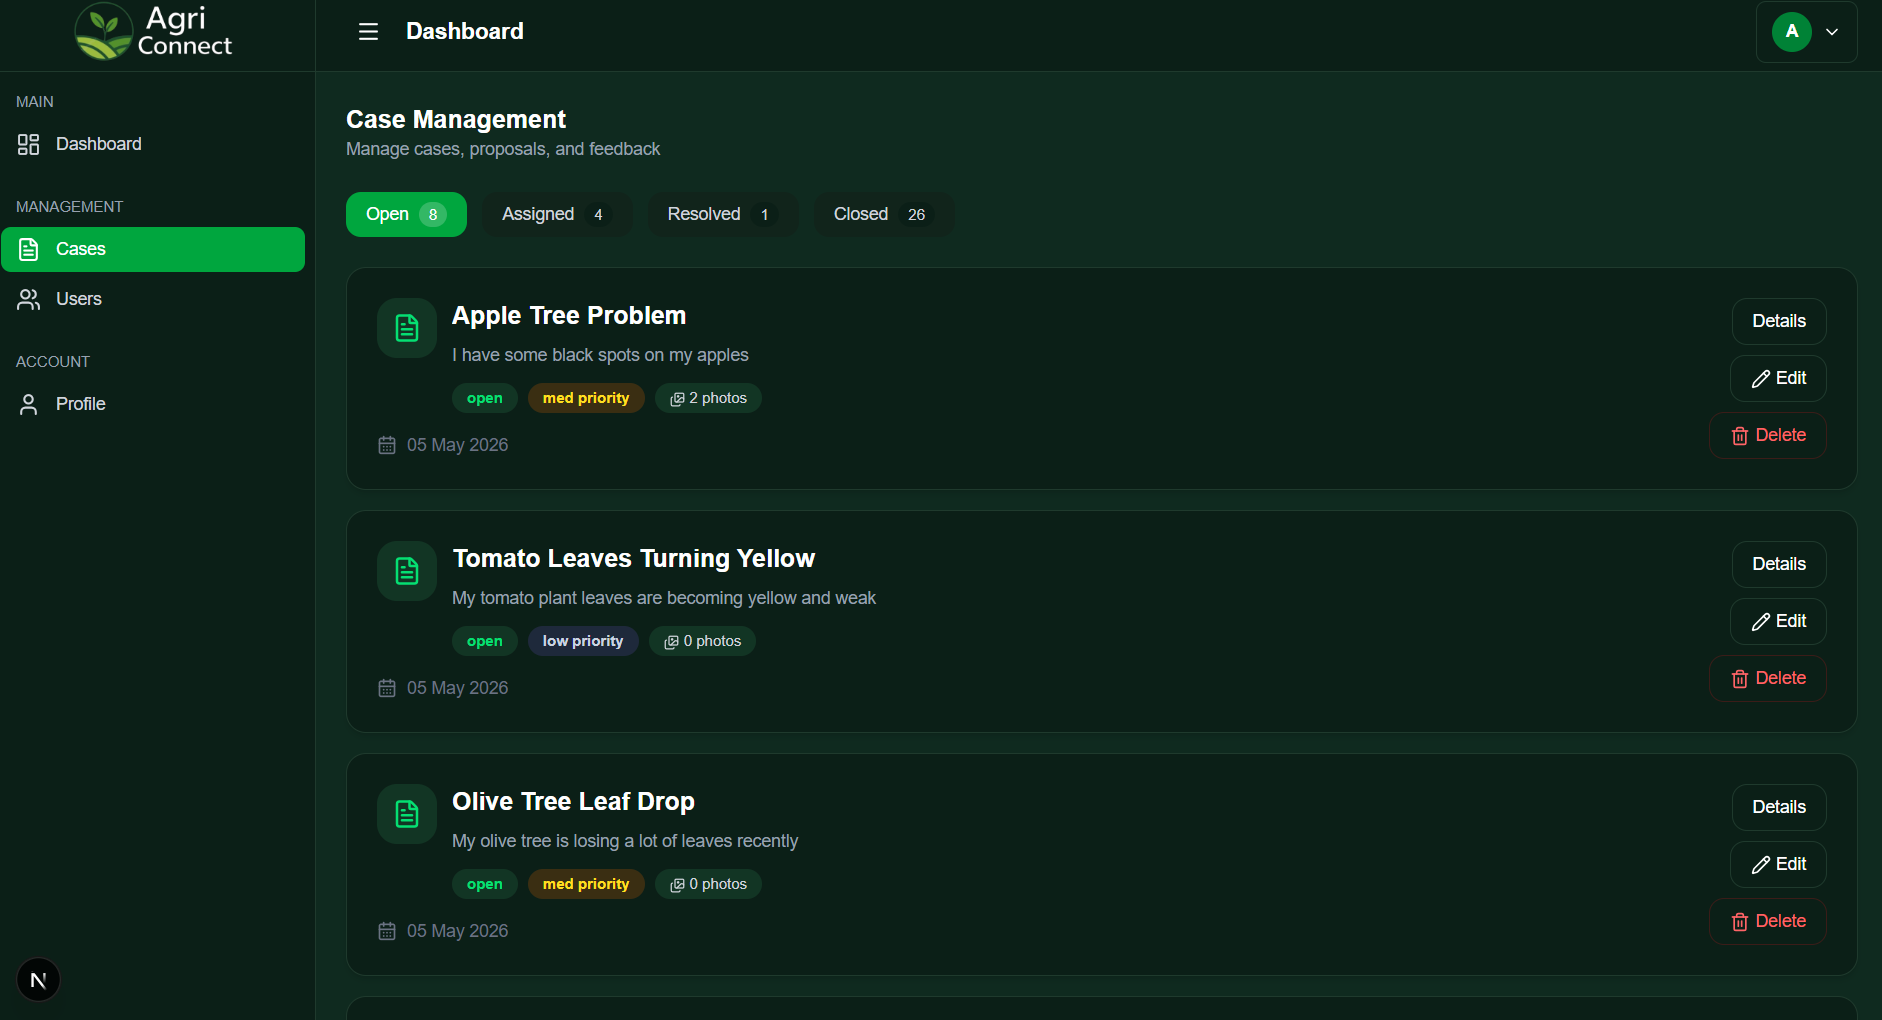
\includegraphics[width=0.9\textwidth]{images/interfaces/admin/admin_cases.png}
\caption{Admin case management interface with status-based organization}
\end{figure}

When accessing case details, the interface is structured into three main sections:

\begin{itemize}
    \item \textbf{Details:} displays complete information about the case, including description and associated images.
    \item \textbf{Proposals:} allows administrators to view, edit, or delete proposals submitted by agronomists.
    \item \textbf{Feedback:} enables management of feedback associated with the case, including editing or deletion.
\end{itemize}

\subsubsection*{User Management}

The user management section allows administrators to supervise all registered users. It is divided into two main categories:

\begin{itemize}
    \item \textbf{Farmers}
    \item \textbf{Agronomists}
\end{itemize}

Administrators can search users by name, email, or phone number. They also have the ability to edit user information or deactivate accounts when necessary.

\begin{figure}[H]
\centering
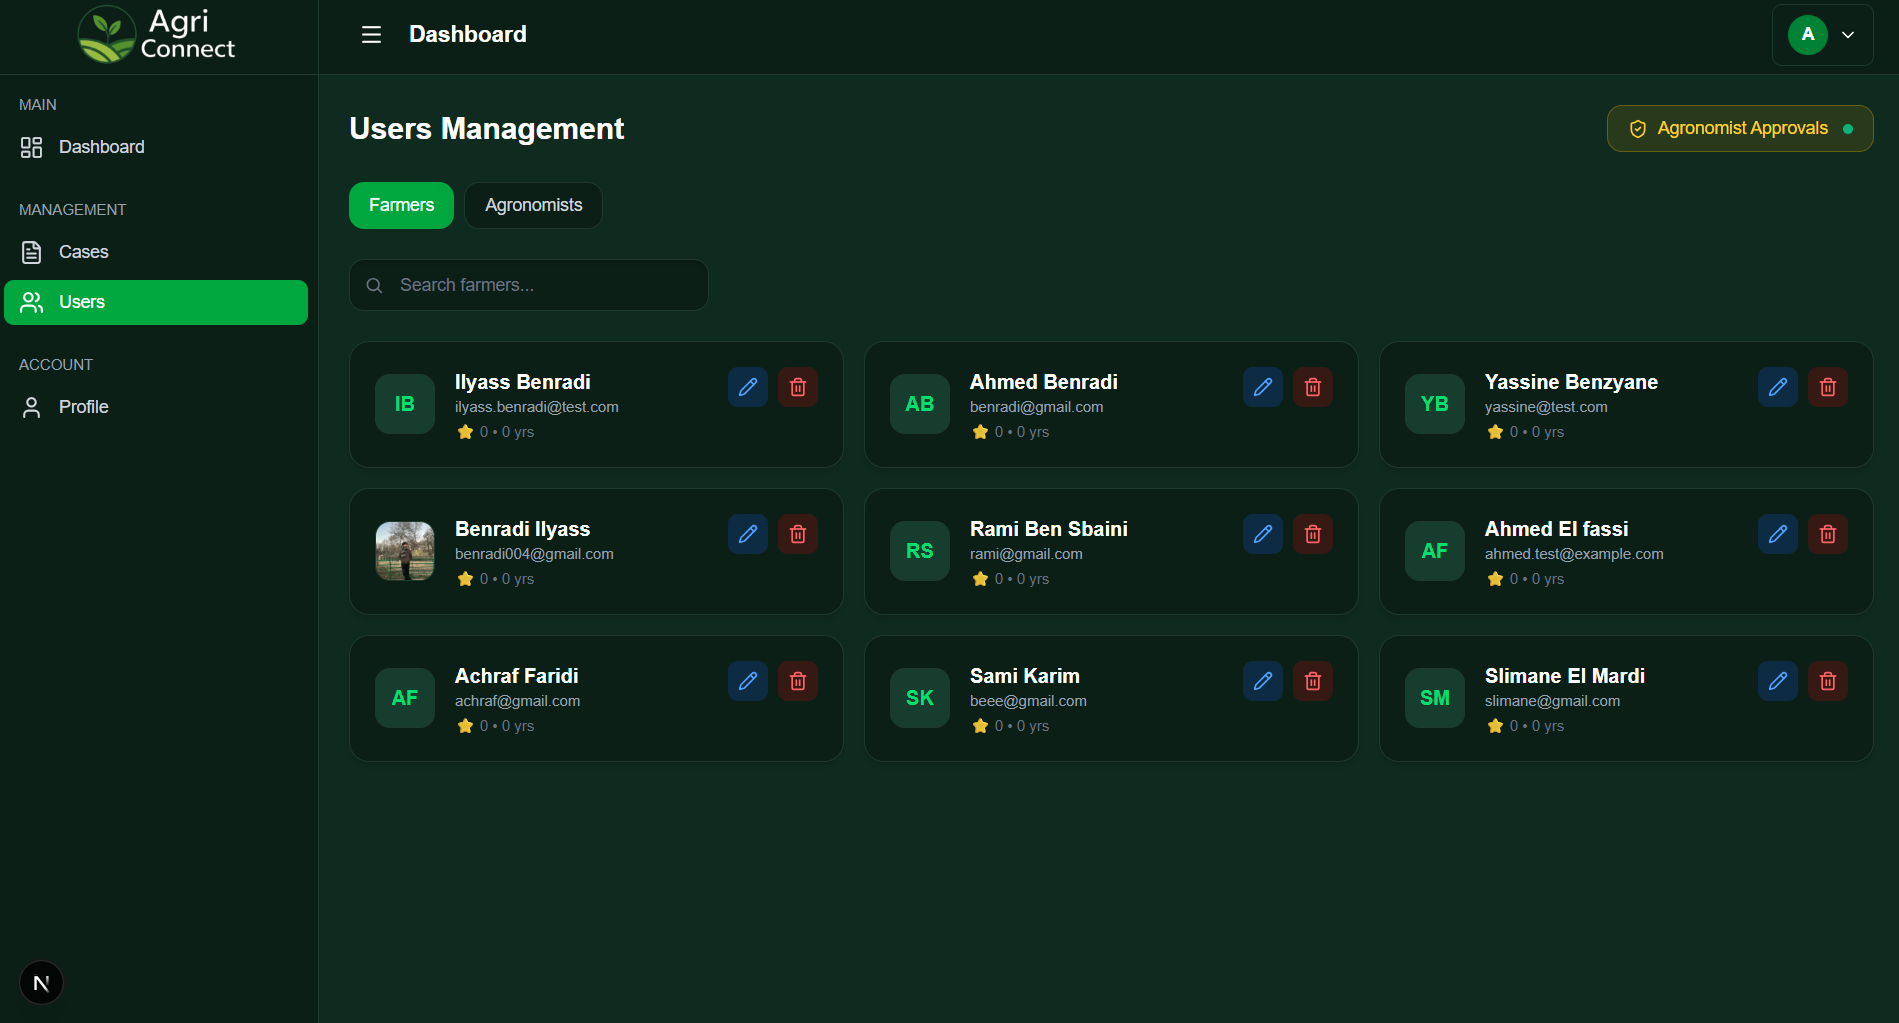
\includegraphics[width=0.9\textwidth]{images/interfaces/admin/admin_users.png}
\caption{Admin user management interface}
\end{figure}

\subsubsection*{Profile and Security}

The admin interface includes a profile management section where administrators can update their account information, such as name and email.

A dedicated security section allows administrators to update their password, ensuring secure access to the platform.

Overall, the admin dashboard provides a comprehensive set of tools for monitoring system activity, managing users and cases, and maintaining the integrity of the platform.




\section{Knowledge Base}

\section{Chapter Summary}

This chapter detailed the implementation of the AgriConnect system, highlighting how the theoretical design was transformed into a functional platform.

The development environment and tools provided the necessary foundation for building the system, while the database implementation ensured structured and efficient data management. The integration of WhatsApp enabled a natural and accessible communication channel for farmers, making the system easy to use in real-world conditions.

The implementation of automated workflows played a crucial role in managing the system’s logic, from message reception and processing to orchestration and knowledge base ingestion. These workflows ensure smooth data flow and coordination between different components of the system.

Furthermore, the multi-agent architecture allowed the system to handle complex tasks by distributing responsibilities across specialized agents, improving modularity and scalability.

The web application complemented the WhatsApp interface by offering advanced functionalities for different users, including case tracking, management, and administration, thus enhancing the overall usability of the platform.

Finally, the knowledge base component enabled intelligent information retrieval, contributing to more accurate and context-aware responses.

In conclusion, the realization phase successfully integrates all components into a coherent system, demonstrating the feasibility and effectiveness of the proposed AgriConnect solution.